\chapter{PENGENDALIAN PENYAKIT}
Pengendalian penyakit sebagai upaya penurunan insiden, prevalensi, morbiditas atau mortalitas dari suatu penyakit, mempunyai peranan penting untuk mengukur derajat kesehatan masyarakat. Pengendalian penyakit menular meliputi penyakit menular langsung, penyakit yang dapat dikendalikan dengan imunisasi dan penyakit yang ditularkan melalui binatang. Sedangkan pengendalian penyakit tidak menular meliputi upaya pencegahan dan deteksi dini penyakit tidak menular tertentu.

\section{PENYAKIT TERBANYAK}
Peringkat pertama penyakit terbanyak di Kabupaten Belitung Timur pada Tahun \tP yang tercatat di keseluruhan Puskesmas adalah Penyakit Tekanan Darah Tinggi/ Hipertensi primer, sebanyak 8.956 kasus (\autoref{fig:10-penyakit-terbanyak}).
Sedangkan peringkat ke-sepuluh adalah Non-insulin-dependent diabetes
mellitus, sebanyak 511 kasus.

\begin{figure}[H]
    \centering
    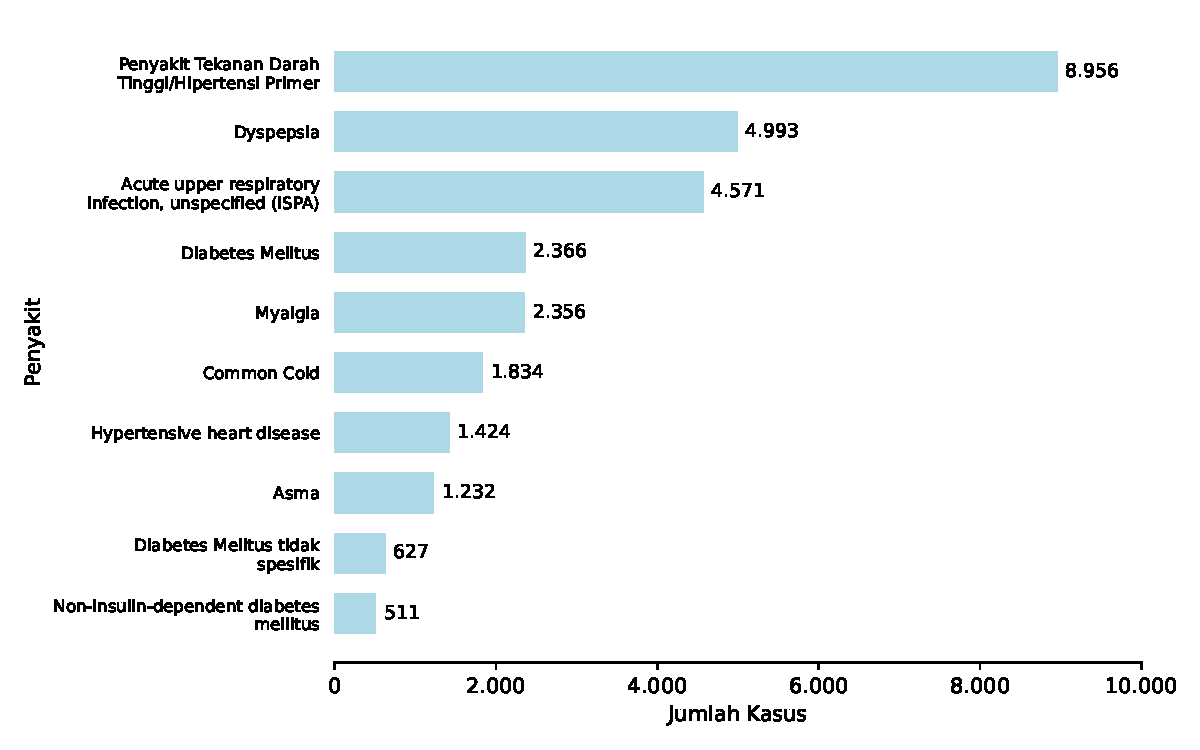
\includegraphics[width=\textwidth]{bab_06/bab_06_00_penyakitTerbanyak}
    \caption{Jumlah 10 Penyakit Terbanyak di Kab. Belitung Timur Tahun \tP}
    \label{fig:10-penyakit-terbanyak}
\end{figure}

\section[PENGENDALIAN PM]{PENGENDALIAN PENYAKIT MENULAR LANGSUNG}
Pengendalian penyakit menular lebih ditekankan pada pelaksanaan surveilans dan epidemologi dengan upaya penemuan penderita secara dini yang ditindaklanjuti dengan penanganan secara cepat. Di samping itu pelayanan lain yang diberikan adalah pemberian imunisasi, upaya penanggulangan faktor resiko melalui program peningkatan kualitas lingkungan serta peningkatan peran serta masyarakat dalam upaya pemberantasan penyakit menular yang dilaksanakan dengan berbagai bentuk kegiatan.

\subsection{Penyakit TB Paru}
Tuberkulosis (TB) Paru merupakan penyakit menular langsung yang disebabkan oleh infeksi bakteri \emph{Mycobacterium tuberculosis} yang menyerang jaringan paru. Gejala utama yaitu batuk berdahak selama 2-3 minggu atau lebih.

\emph{Treatment Coverage} TBC adalah jumlah semua kasus tuberkulosis yang ditemukan dan diobati di antara perkiraan jumlah semua kasus tuberkulosis (insiden
tuberkulosis). Pada tahun \tP terdapat 266 kasus TB di Kabupaten Belitung Timur (\autoref{fig:Jumlah-Kasus-TB}) sehingga TC TB pada tahun \tP adalah sebesar 44,28\%.

\begin{figure}[H]
  \centering
  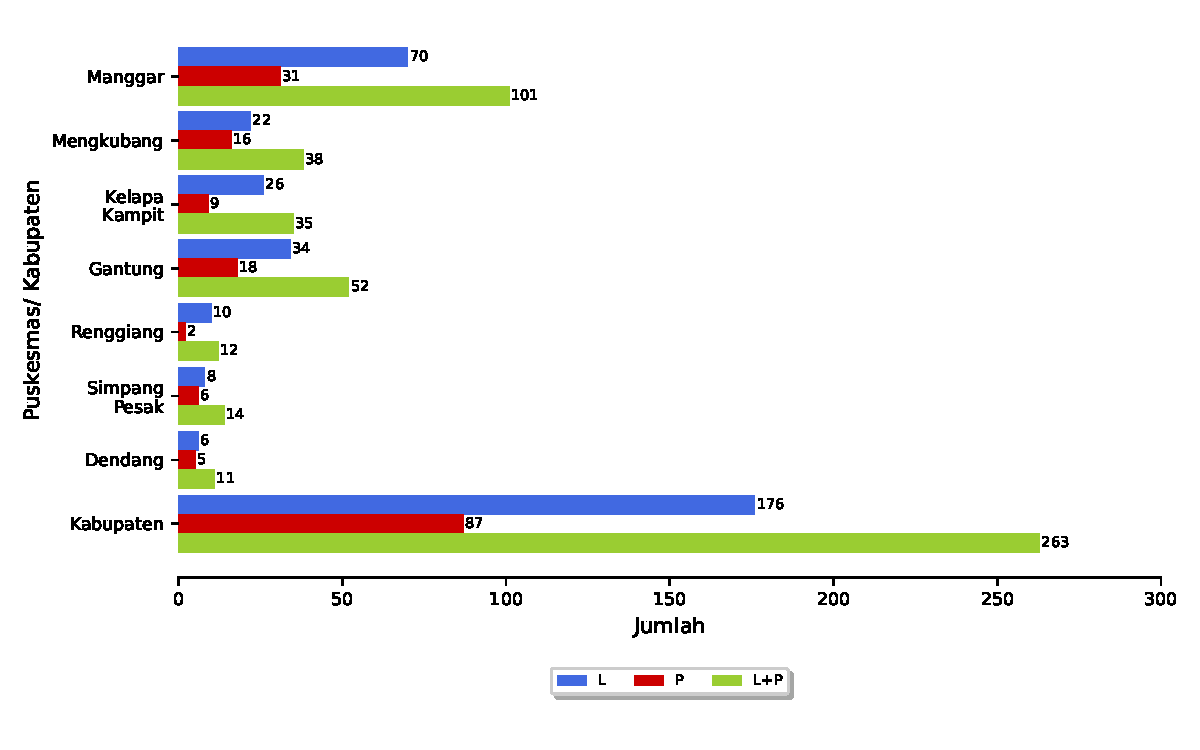
\includegraphics[width=0.85\textwidth]{bab_06/bab_06_01a_kasusTB}
  \caption{Jumlah Kasus TB di Kab. Belitung Timur Tahun \tP per Puskesmas}
  \label{fig:Jumlah-Kasus-TB}
\end{figure}

Cakupan penemuan TB anak adalah jumlah seluruh kasus tuberkulosis anak yang ditemukan di antara perkiraan jumlah kasus tuberkulosis anak yang ada disuatu wilayah dalam periode tertentu. Perkiraan jumlah kasus tuberkulosis  anak adalah 12\% dari perkiraan jumlah semua kasus TB (insiden) yang ada di masing-masing kabupaten/ kota. Jumlah kasus TB anak pada tahun \tP adalah sebanyak 54 kasus, sehingga cakupan penemuan TB anak adalah sebesar 72,35\%.

\begin{figure}[H]
    \centering
    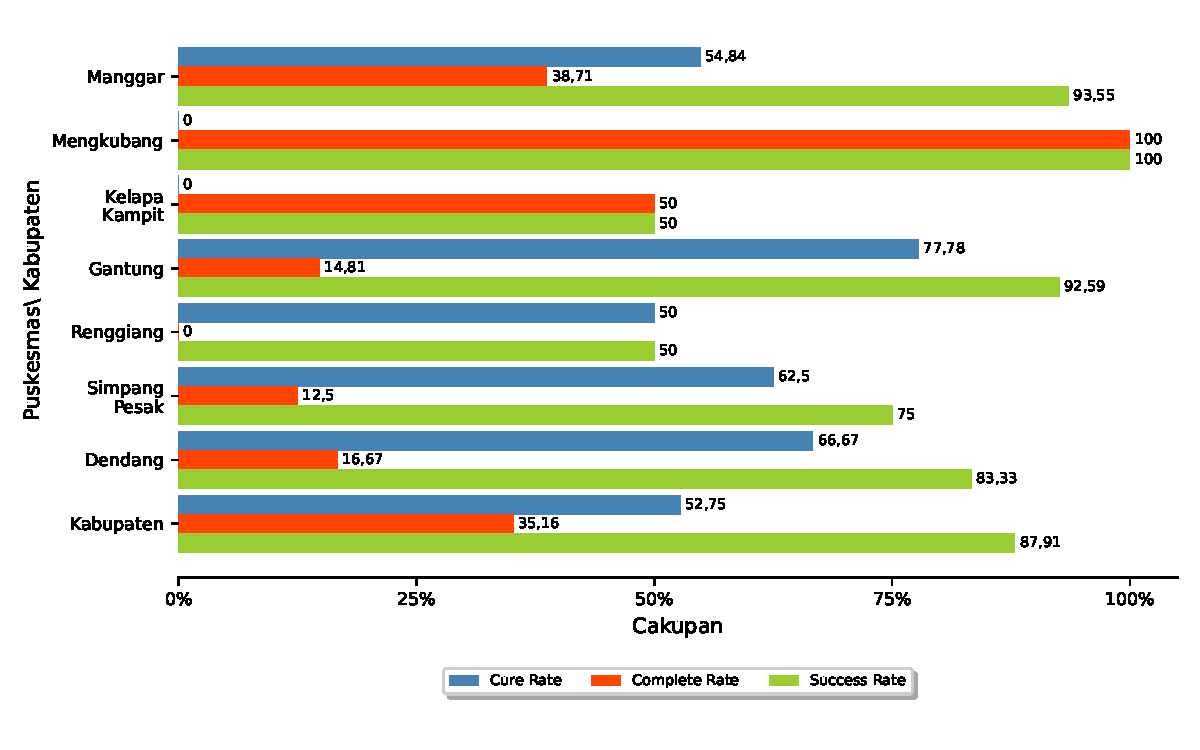
\includegraphics[width=0.85\textwidth]{bab_06/bab_06_01b_cureCompSuccRateTB}
    \caption{\emph{Cure Rate} \& \emph{Success Rate} TB paru di Kab. Belitung Timur Tahun \tP per Puskesmas}
    \label{fig:Cure-Rate-TB}
\end{figure}

Upaya pencegahan dan pemberantasan TB-Paru dilakukan dengan pendekatan
DOTS (\emph{Directly Observe Treatment Shortcourse}) atau pengobatan TB-Paru
dengan pengawasan langsung oleh Pengawas Menelan Obat (PMO). Kegiatan
ini berupaya menemukan penderita dengan pemeriksaan dahak di sarana
pelayanan kesehatan yang ditindaklanjuti dengan paket pengobatan.

Angka Kesembuhan (\emph{Cure Rate}) TB paru terkonfirmasi biologis adalah jumlah pasien TB paru terkonfirmasi biologis yang sembuh di suatu wilayah pada kohort yang sama dengan hasil pemeriksaan bakteriologis pada akhir pengobatan menjadi negatif dan pada salah satu pemeriksaan sebelumnya.
\emph{Cure Rate} pada tahun \tP di Kabupaten Belitung Timur adalah sebanyak 48 orang (52,75\%).

Angka Pengobatan Lengkap (\emph{Complete Rate}) TB adalah jumlan pasien tuberkulosis yang telah menyelesaikan pengobatan secara lengkap dimana pada salah satu pemeriksaan sebelum akhir pengobatan hasilnya negatif namun tanpa ada bukti hasil pemeriksaan bakteriologis pada akhir pengobatan.
\emph{Complete Rate} pada tahun \tP di Kabupaten Belitung Timur adalah sebanyak 32 orang (35,16\%).

Angka Keberhasilan Pengobatan (\emph{Success Rate}) TBadalah jumlah pasien tuberkulosis semua kasus yang sembuh dan pengobatan lengkap diantara semua kasus tuberkulosis yang diobati dan dilaporkan.
\emph{Success Rate} pada tahun \tP di Kabupaten Belitung Timur adalah sebanyak 80 orang (87,91\%).

Terdapat 6 kasus kematian akibat TB di Kabupaten Belitung Timur pada tahun \tPnos atau 6,59\% dari jumlah kasus.

\begin{figure}[H]
	\centering
	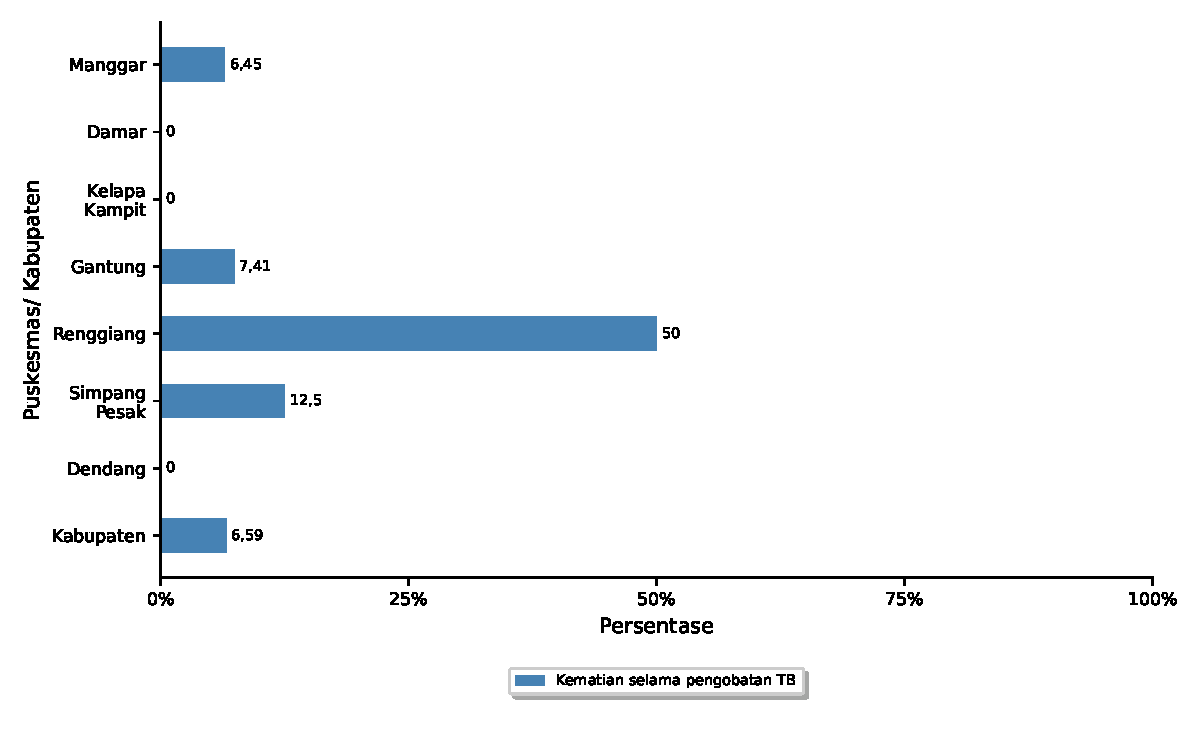
\includegraphics[width=0.85\textwidth]{bab_06/bab_06_01c_kematianTB}
	\caption{Kematian pada pengobatan TB paru di Kab. Belitung Timur Tahun \tP per Puskesmas}
	\label{fig:kematian-TB}
\end{figure}

\subsection{Penyakit Pneumonia}
Pneumonia balita adalah balita mengalami batuk dan atau kesukaran bernapas dan hasil perhitungan napas, usia 0-2 bulan $\geq$60 kali/menit, usia 2-12 bulan $\geq$ 50 kali/menit, usia 12-59 bulan $\geq$ 40 kali/menit. Pneumonia berat jika balita mengalami tarikan dinding dada ke dalam (TDDK) atau saturasi oksigen $<$ 90.\

Tatalaksana pneumonia sesuai standar adalah jika balita dengan keluhan batuk dan atau kesukaran bernafas yang berkunjung ke sarana kesehatan diberikan tatalaksana standar dilakukan hitung napas/ melihat TDDK. Cakupan tatalaksana pneumonia sesuai standar di Kabupaten Belitung Timur pada tahun \tP adalah sebesar 99,79\% (\autoref{fig:Penemuan-Pneumonia-Balita}).

Penemuan penderita pneumonia balita adalah cakupan balita dengan pneumonia yang ditemukan dan diberikan tatalaksana sesuai standar di sarana kesehatan di satu wilayah dalam waktu satu tahun. Penemuan kasus penumonia balita di Kabupaten Belitung Timur pada tahun \tP adalah sebesar 10,92\% dari target penemuan.

\begin{figure}[H]
    \centering
    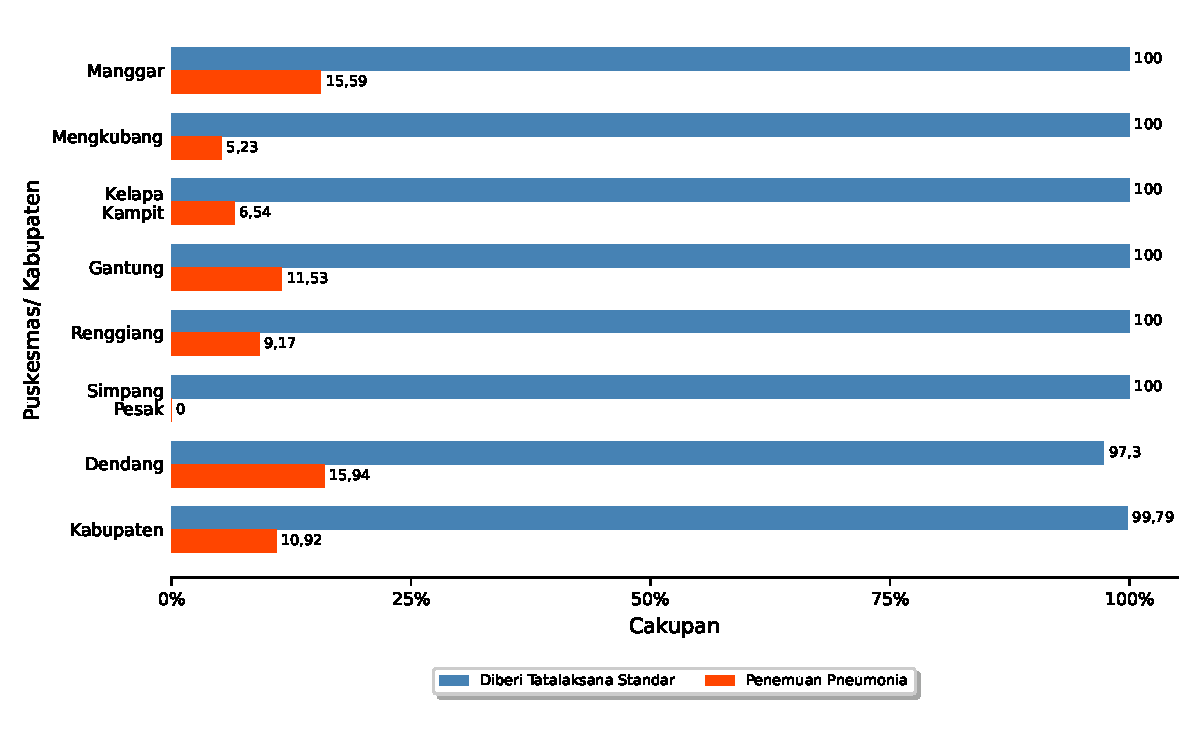
\includegraphics[width=0.9\textwidth]{bab_06/bab_06_02_pneumoniaBalita}
    \caption{Cakupan Penanganan dan Penemuan Pneumonia Pada Balita di Kab. Belitung Timur Tahun \tP per Puskesmas}
    \label{fig:Penemuan-Pneumonia-Balita}
\end{figure}


\subsection{Penyakit HIV/ AIDS}
HIV/ AIDS merupakan penyakit menular yang disebabkan oleh infeksi
\emph{Human Immunodeficiency Virus} yang menyerang sistem kekebalan tubuh.
Infeksi tersebut menyebabkan penderita mengalami penurunan ketahanan
tubuh sehingga sangat mudah untuk terinfeksi berbagai macam penyakit
lain.

Pelayanan kesehatan yang diberikan kepada orang dengan risiko terinfeksi virus HIV meliputi: pemberian komunikasi, informasi, dan edukasi (KIE) tentang HIV termasuk promosi kesehatan penggunaan alat pencegahan yang efektif (kondom, lubrikan (pelumas), alat suntik steril, dll); pelayanan pemeriksaan laboratorium berupa skrining (deteksi dini) HIV, dan pelayanan konfirmasi diagnosis rujukan ke layanan pengobatan Anti Retroviral (ARV). Sedangkan yang termasuk orang dengan resiko terinfeksi HIV adalah:
\begin{enumerate}
  \item Ibu hamil;
  \item Pasien TBC;
  \item Pasien Infeksi Menular Seksual (IMS);
  \item Penjaja seks;
  \item Lelaki yang berhubungan seks dengan lelaki (LSL);
  \item Transgender/Waria;
  \item Pengguna napza suntik (penasun);
  \item Warga Binaan Pemasyarakatan; dan
  \item Kelompok rentan.
\end{enumerate}

Jumlah Kasus HIV di Kabupaten Belitung Timur tahun \tP adalah sebanyak 0 kasus (\autoref{fig:Jumlah-Kasus-HIV}), sedangkan cakupan pelayanan deteksi dini HIV di Kabupaten Belitung Timur pada tahun \tP adalah sebesar 93,81\%.

\begin{figure}[H]
  \centering
  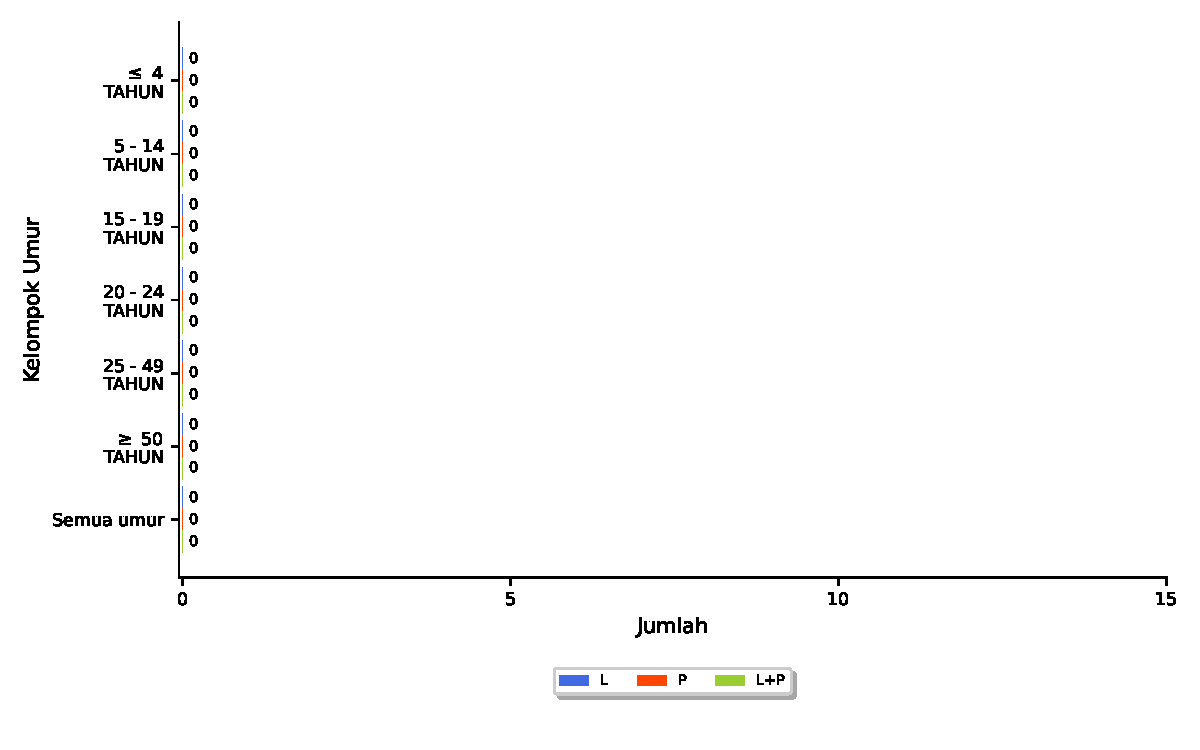
\includegraphics[width=0.85\textwidth]{bab_06/bab_06_03a_HIV}
  \caption{Jumlah Kasus HIV Kab. Belitung Timur Tahun \tP}
  \label{fig:Jumlah-Kasus-HIV}
\end{figure}

Antiretroviral (ARV) merupakan bagian dari pengobatan HIV dan AIDS untuk mengurangi risiko penularan HIV, menghambat perburukan infeksi oportunistik, meningkatkan kualitas hidup penderita HIV, dan menurunkan jumlah virus (\emph{viral load}) dalam darah sampai tidak terdeteksi. Cakupan orang dengan HIV (ODHIV) baru yang mendapat pengobatan ARV di Kabupaten Belitung Timur pada tahun \tP adalah sebesar 73,08\%.

\begin{figure}[H]
  \centering
  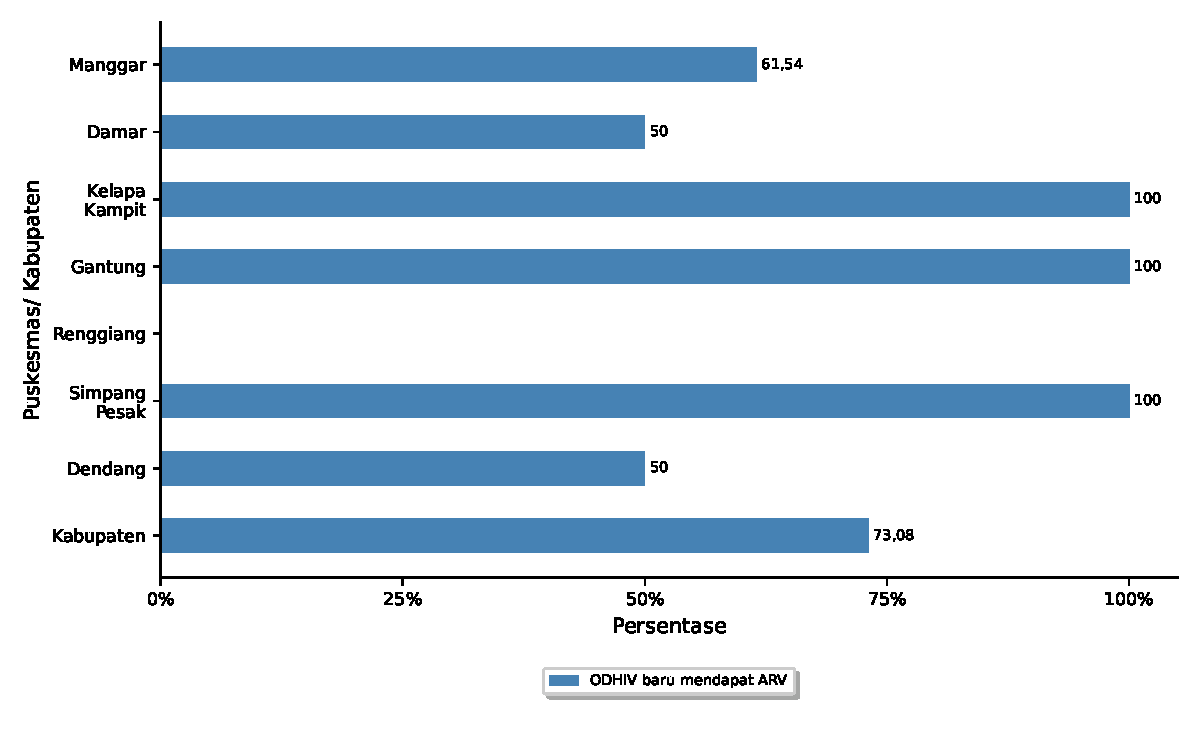
\includegraphics[width=0.85\textwidth]{bab_06/bab_06_03b_ARV}
  \caption{ODHIV ARV Kab. Belitung Timur Tahun \tP}
  \label{fig:HIV-ARV}
\end{figure}

Upaya pelayanan kesehatan dalam rangka penanggulangan HIV/AIDS di samping ditujukan pada penanganan penderita yang ditemukan juga diupayakan pada pencegahan melalui penemuan penderita secara dini yang dilanjutkan dengan konseling.
Kegiatan yang telah dilaksanakan di Kabupaten Belitung Timur tahun \tP dalam rangka penurunan angka kesakitan akibat HIV/AIDS dan PMS antara lain adalah Penyebaran Informasi (KIE) HIV/AIDS, Sero Survei HIV/AIDS, Skrining Darah, serta Monitoring dan Evaluasi HIV/AIDS.

\subsection{Penyakit Diare}
Diare adalah suatu penyakit yang ditandai dengan perubahan bentuk dan konsistensi tinja yang lembek sampai mencair dan bertambahnya frekuensi buang air besar yang lebih dari biasa, yaitu 3 kali atau lebih dalam sehari yang mungkin dapat disertai dengan muntah atau tinja yang berdarah.
Penyebab diare dikelompokkan dalam 6 golongan besar, yaitu infeksi (bakteri/ virus/ parasit), malabsorpsi, alergi, keracunan, imunodefisiensi dan sebab-sebab lainnya. Diare biasanya berlangsung beberapa hari, namun sebagian kasus dapat memanjang hingga beberapa minggu.
Diare dapat menyebabkan kematian; publikasi WHO pada tahun 2009 menunjukkan diare adalah penyebab kedua terbanyak kematian pada balita secara global.

Jumlah perkiraan kasus diare tahun \tP di Kabupaten Belitung Timur sebanyak 1.582 kasus balita dan 3.484 kasus semua umur.
Jumlah kasus yang ditemukan sebesar 304 kasus balita (19,22\%) dan 1.032 kasus semua umur (29,62\%) (\autoref{fig:Cakupan-Kasus-Diare-Dilayani}).

\begin{figure}[H]
    \centering{}
    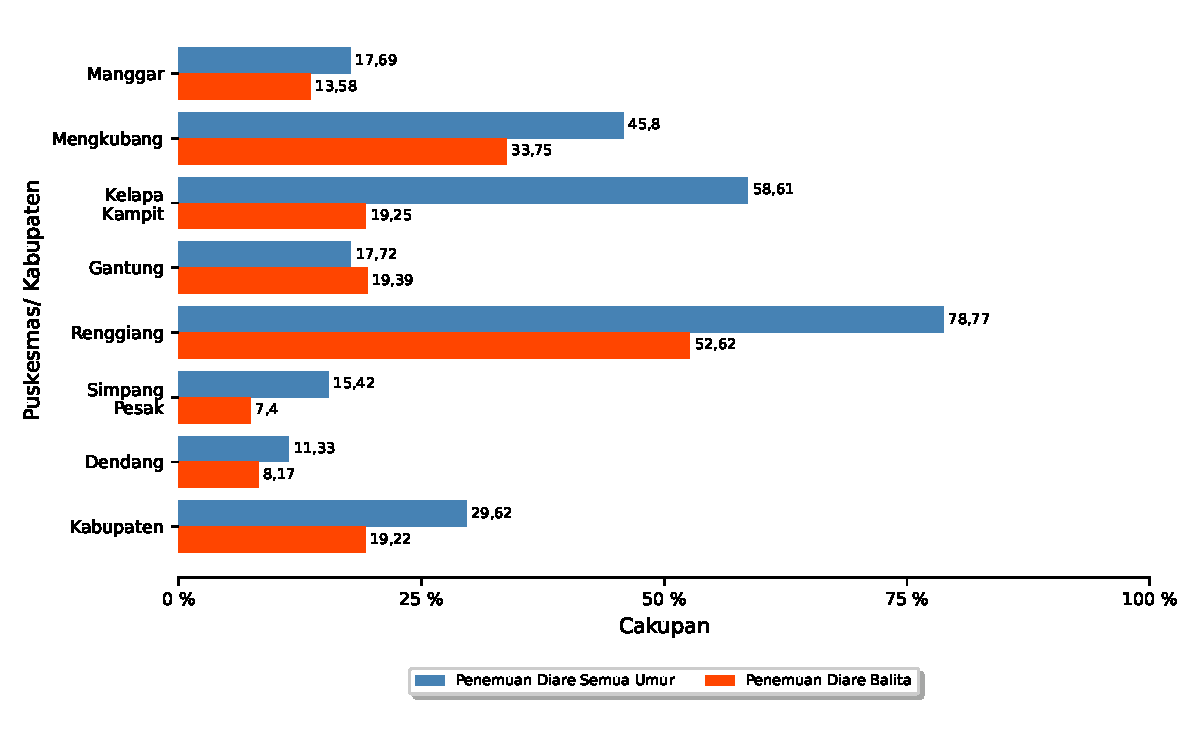
\includegraphics[width=0.9\textwidth]{bab_06/bab_06_04a_diareDilayani}
    \caption{Cakupan Penanganan Kasus Diare di Kab. Belitung Timur Tahun \tP per Puskesmas}
    \label{fig:Cakupan-Kasus-Diare-Dilayani}
\end{figure}

\begin{figure}[H]
	\centering{}
	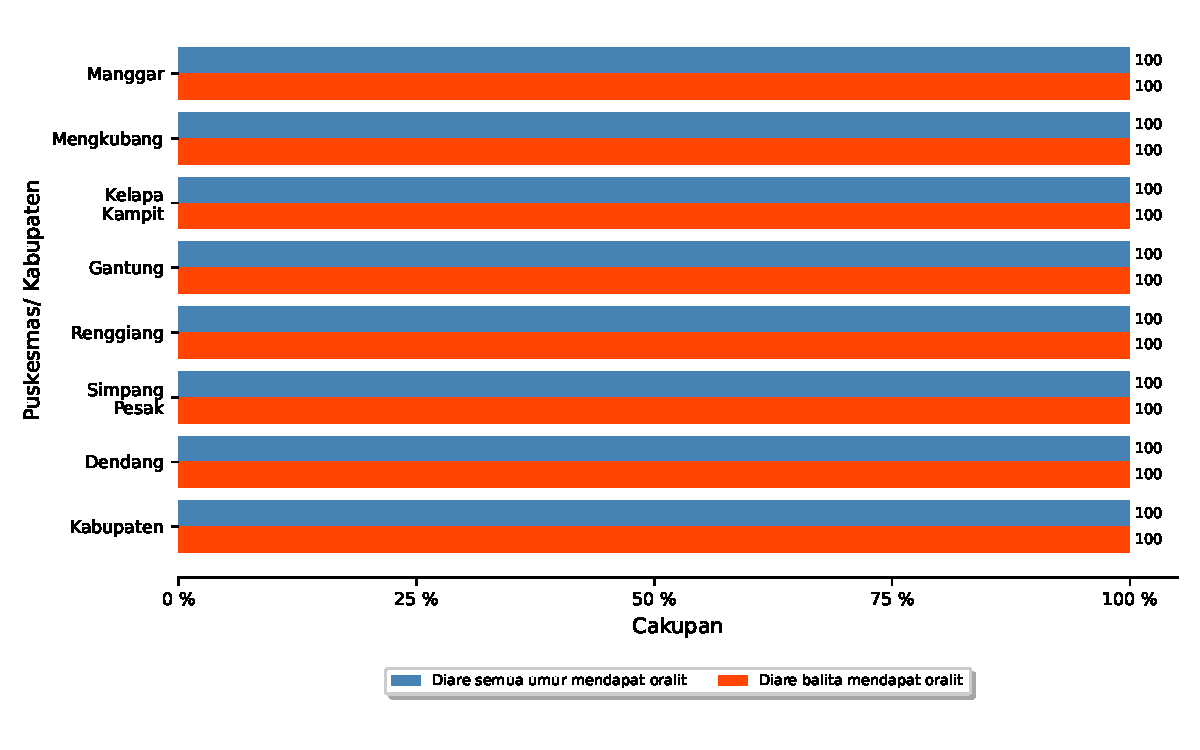
\includegraphics[width=0.9\textwidth]{bab_06/bab_06_04b_diareOralit}
	\caption{Cakupan Kasus Diare Diberi Oralit di Kab. Belitung Timur Tahun \tP per Puskesmas}
	\label{fig:Cakupan-Kasus-Diare-Oralit}
\end{figure}

\begin{figure}[H]
	\centering{}
	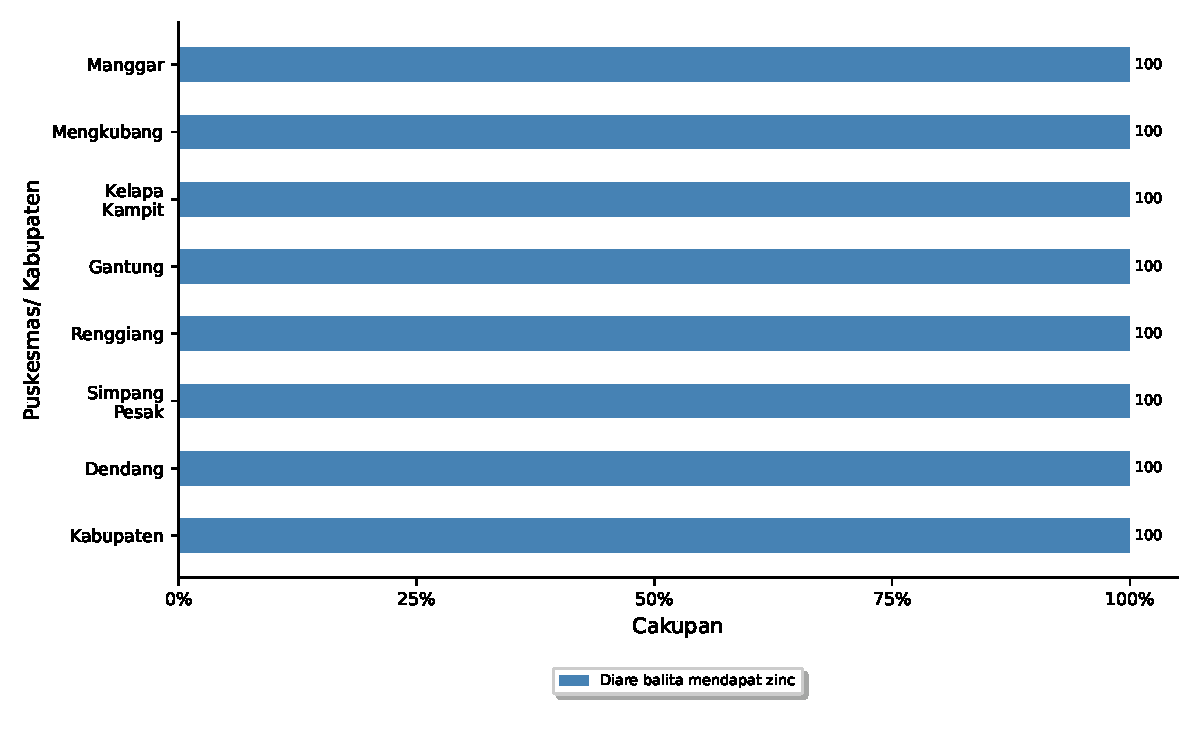
\includegraphics[width=0.9\textwidth]{bab_06/bab_06_04c_diareZinc}
	\caption{Cakupan Kasus Diare Diberi Zinc di Kab. Belitung Timur Tahun \tP per Puskesmas}
	\label{fig:Cakupan-Kasus-Diare-Zinc}
\end{figure}

\subsection{Deteksi Hepatitis B}
Hepatitis B adalah penyakit menular dalam bentuk peradangan hati yang disebabkan oleh virus Hepatitis B. Virus Hepatitis B menyebar melalui darah atau cairan tubuh. Di Indonesia, penularan Hepatitis B umumnya terjadi pada bayi pada saat proses kelahirannya. Deteksi dini Hepatitis B pada ibu hamil dapat membantu memitigasi penularan virus dari ibu ke bayi. Deteksi dini Hepatitis B dilakukan melalui pemeriksaan HBsAg. HBsAg (\emph{Hepatitis B Surface Antigen}) merupakan antigen permukaan yang ditemukan pada virus hepatitis B yang memberikan arti adanya infeksi hepatitis B.

Cakupan deteksi dini Hepatitis B pada ibu hamil di Kabupaten Belitung Timur pada tahun \tP adalah sebesar 83,33\% , dan ditemukan 2,33\% ibu hamil menunjukkan hasil reaktif.

\begin{figure}[H]
	\centering{}
	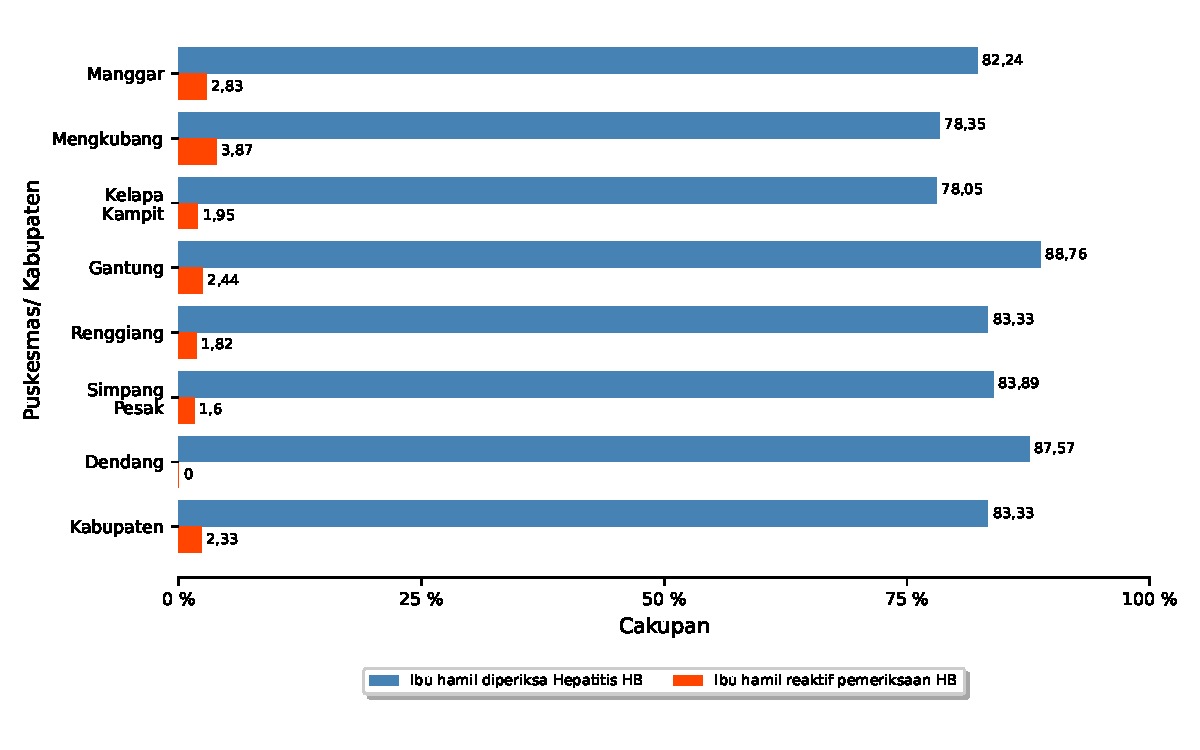
\includegraphics[width=0.9\textwidth]{bab_06/bab_06_05a_bumilHB}
	\caption{Cakupan Deteksi Hepatitis B pada Ibu Hamil di Kab. Belitung Timur Tahun \tP per Puskesmas}
	\label{fig:Cakupan-Bumil-HB}
\end{figure}

HBIg (\emph{Hepatitis B Immunoglubulin}) merupakan serum antibodi spesifik Hepatitis B yang memberikan perlindungan langsung kepada bayi yang lahir dari ibu dengan HBSAg reaktif (positif). HBIg efektif diberikan kepada bayi sebelum 24 jam setelah lahir.

Cakupan bayi lahir dari ibu yang reaktif HBsAg mendapat HBIG di Kabupaten Belitung Timur pada tahun \tP adalah sebesar 100\% .

\begin{figure}[H]
	\centering{}
	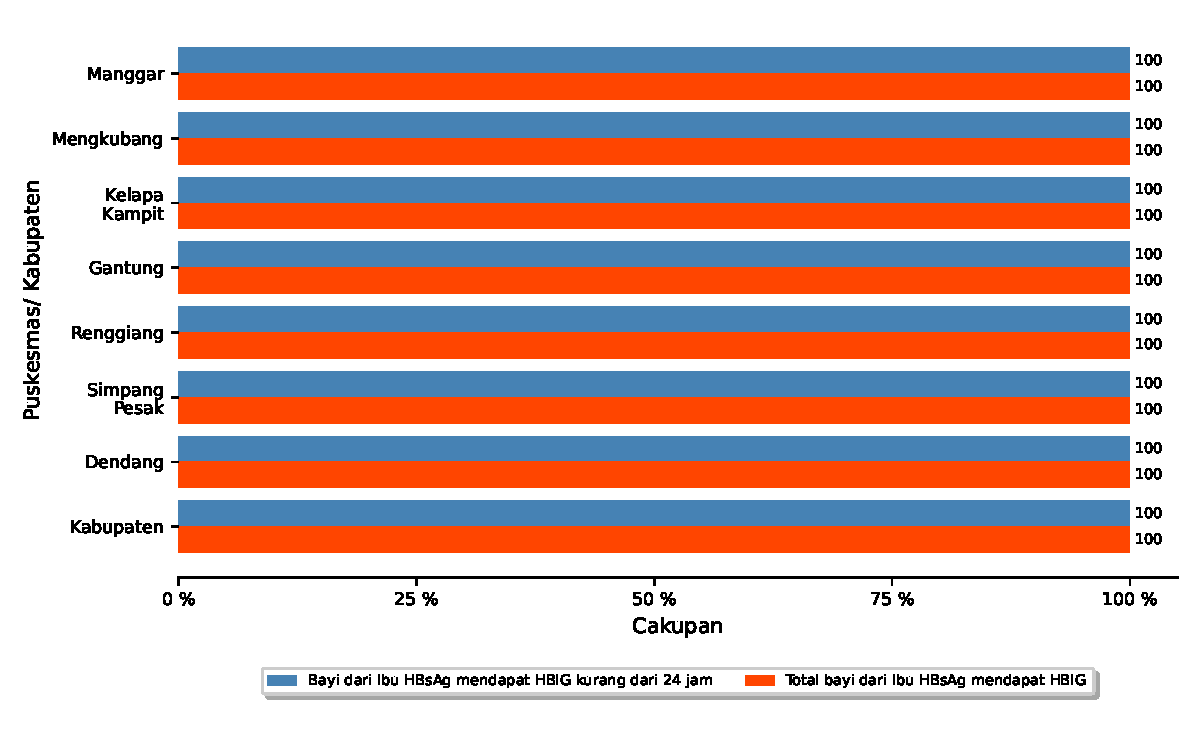
\includegraphics[width=0.9\textwidth]{bab_06/bab_06_05b_bayiHBIG}
	\caption{Cakupan Deteksi Hepatitis B pada Bayi di Kab. Belitung Timur Tahun \tP per Puskesmas}
	\label{fig:Cakupan-Bayi-HBIG}
\end{figure}

\subsection{Penyakit Kusta}
Kusta adalah sebuah penyakit infeksi kronis yang disebabkan oleh bakteri \emph{Mycobacterium leprae} yang menyerang saraf tepi dan kulit.
Gejala kusta antara lain rasa kesemutan pada anggota badan atau raut muka dan mati rasa pada kulit karena kerusakan saraf tepi.
Penanganan kusta yang terlambat dapat menyebabkan kerusakan pada kulit, saraf-saraf, anggota gerak dan mata dengan sangat progresif.

Kusta terbagi atas dua macam yaitu Kusta Kering/ Pausi Basiler (PB) dan Kusta Basah/ Multi Basiler (MB).
PB memiliki tanda utama jumlah bercak kusta 1-5, jumlah penebalan saraf tepi disertai gangguan fungsi hanya 1 saraf, dan hsil pemeriksaan kerokan jaringan kulit negatif.
Sedangkan MB memiliki tanda utama jumlah bercak kusta $>$ 5, jumlah penebalan saraf tepi disertai gangguan fungsi lebih dari 1 saraf, dan hasil pemeriksaan kerokan jaringan kulit positif.

Meskipun Indonesia sudah mencapai eliminasi Kusta mulai dari tahun 2000, akan tetapi penyakit Kusta masih merupakan salah satu masalah penyakit yang ada di masyarakat.

Jumlah kasus baru kusta di Kabupaten Belitung Timur pada tahun \tP berjumlah 5 kasus (\autoref{fig:Jumlah-Kasus-Baru-Kusta}).
Angka penemuan kasus baru/ \emph{New Case Detection Rate} (NCDR) adalah sebesar 3,87 per 100.000 penduduk.

\begin{figure}[H]
  \centering
  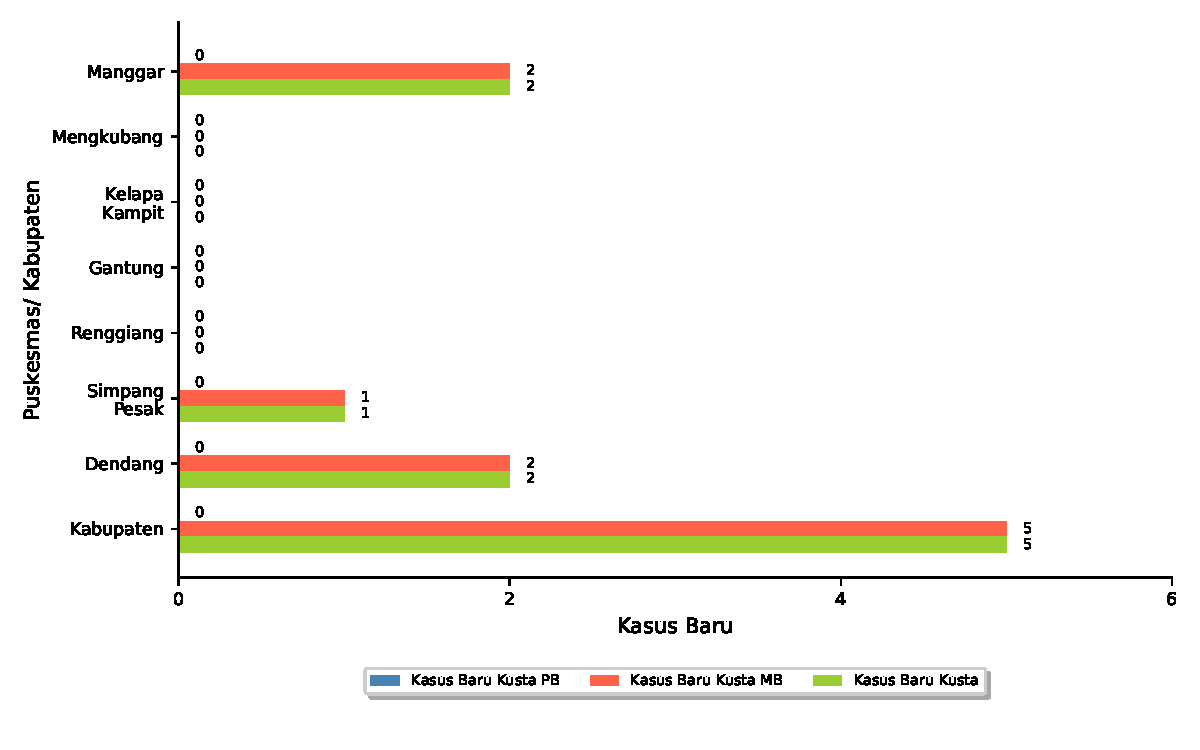
\includegraphics[width=0.9\textwidth]{bab_06/bab_06_06a_kasusBaruKusta}
  \caption{Jumlah Kasus Baru Kusta di Kab. Belitung Timur Tahun \tP}
  \label{fig:Jumlah-Kasus-Baru-Kusta}
\end{figure}

Jumlah kasus kusta terdaftar di Kabupaten Belitung Timur pada tahun \tP berjumlah 5 kasus (\autoref{fig:Jumlah-Kasus-Terdaftar-Kusta}).
Angka prevalensi kusta adalah sebesar 0,39 per 10.000 penduduk.

\begin{figure}[H]
	\centering
	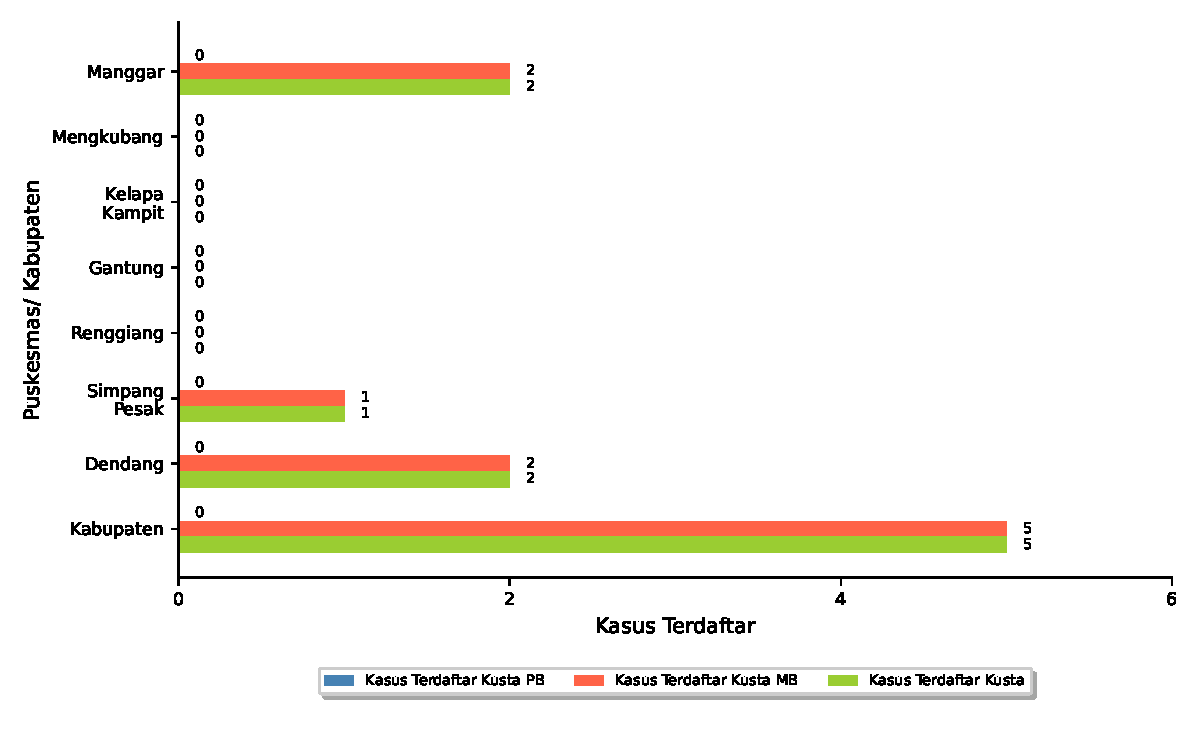
\includegraphics[width=0.9\textwidth]{bab_06/bab_06_06b_kasusTerdaftarKusta}
	\caption{Jumlah Kasus Terdaftar Kusta di Kab. Belitung Timur Tahun \tP}
	\label{fig:Jumlah-Kasus-Terdaftar-Kusta}
\end{figure}

Upaya pelayanan terhadap penderita penyakit kusta antara lain dengan melakukan penemuan penderita melalui survey pada anak sekolah.
Survey kontak dan pemeriksaan intensif penderita yang datang ke tempat pelayanan kesehatan atau kontak dengan penderita penyakit kusta.
Untuk menurunkan angka kesakitan penderita penyakit kusta, kegiatan yang telah dilakukan selama tahun \tP antara lain adalah penemuan penderita secara aktif dan pasif, pengendalian dan pengawasan minum obat, survei penderita kusta, peningkatan kemapuan petugas melaui pelatihan dan pendidikan, rapat koordinasi, evaluasi dan monitoring program kusta.

\emph{Release From Treatment} (RFT) PB adalah jumlah kasus baru PB dari periode kohort satu tahun yang sama yang menyelesaikan pengobatan tepat waktu (6 blister dalam 6-9 bulan).
Sedangkan \emph{Release From Treatment} (RFT) MB adalah jumlah kasus baru MB dari periode kohort satu tahun yang sama yang menyelesaikan pengobatan tepat waktu (12 blister dalam 12-18 bulan).
RFT \emph{rate} PB di Kabupaten Belitung Timur pada tahun \tP adalah nihil karena tidak ada penderita PB pada kohort 2022. Sedangkan RFT \emph{rate} MB di Kabupaten Belitung Timur pada tahun \tP adalah sebesar 100,00\% (\autoref{fig:Cakupan-RFT-Kusta}).

\begin{figure}[H]
  \centering
  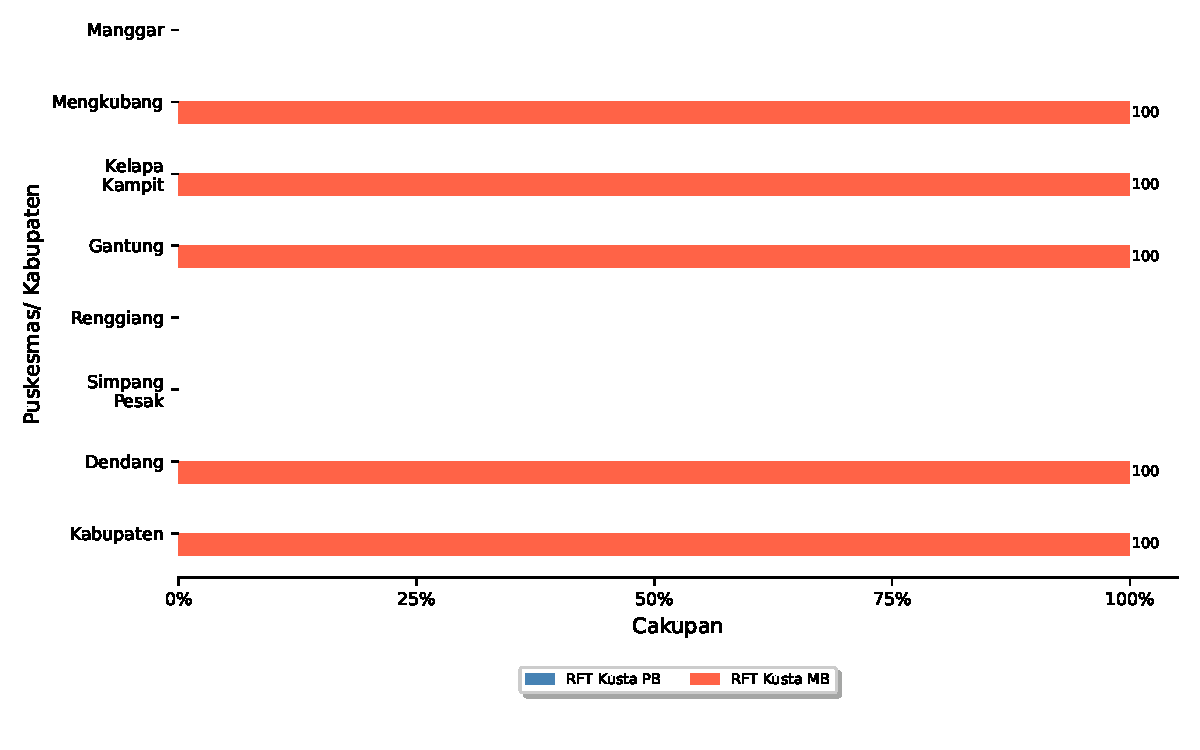
\includegraphics[width=0.85\textwidth]{bab_06/bab_06_06c_RFTkusta}
  \caption{Cakupan \emph{Release From Treatment} (RFT) Kusta di Kab. Belitung Timur Tahun \tP}
  \label{fig:Cakupan-RFT-Kusta}
\end{figure}

\section[PENGENDALIAN PD3I]{PENGENDALIAN PENYAKIT YANG DAPAT DICEGAH DENGAN IMUNISASI}
\subsection{Penyakit Acute Flaccid Paralysis (AFP)}
Upaya pemberantasan dan pencegahan penyakit polio telah dilakukan dengan gerakan Imunisasi Polio.
Upaya ini juga ditindak lanjuti dengan kegiatan surveilans epidemologi secara aktif terhadap kasus-kasus \emph{Acute Flaccid Paralysis} (AFP) kelompok umur < 15 tahun hingga dalam kurun waktu tertentu, untuk mencari kemungkinan adanya virus polio yang berkembang di masyarakat dengan pemeriksaan specimen tinja dari kasus AFP yang dijumpai.
AFP adalah kelumpuhan pada anak berusia $<$15 tahun yang bersifat layuh (\emph{flaccid}) terjadi secara akut/ mendadak ($<$ 14 hari) dan bukan disebabkan oleh rudapaksa (cedera trauma/ \emph{bodily injury or wound}).

Pada tahun \tP ditemukan 0 kasus AFP anak di Kabupaten Belitung Timur, sehingga AFP \emph{rate} adalah 0 per 100.000 penduduk usia $<$ 15 tahun.

\subsection{Penyakit Difteri, Pertusis dan Tetanus}
Difteri adalah penyakit infeksi yang disebabkan oleh kuman \emph{Corynebacterium diphtheria} ditandai dengan adanya peradangan pada tempat infeksi, terutama pada selaput bagian dalam saluran pernapasan bagian atas, hidung dan juga kulit.
Pertusis adalah penyakit menular yang di sebabkan oleh bakteri \emph{Bordetella pertussis} yang menyerang saluran pernafasan dan biasanya terjadi pada anak berusia dibawah 1 tahun.
Tetanus neonatarum adalah penyakit tetanus yang terjadi pada neonatus (0-28 hari) yang disebabkan oleh \emph{Clostridium tetani}, yaitu kuman yang mengeluarkan toksin (racun) dan menyerang sistem saraf pusat.

Pada tahun \tP tidak ditemukan kasus difteri, pertusis ataupun tetanus neonatarum di Kabupaten Belitung Timur.

\subsection{Penyakit Hepatitis B}
Hepatitis B adalah penyakit peradangan pada sel-sel hati, yang disebabkan oleh infeksi virus Hepatitis B dari golongan virus DNA.

Pada tahun \tP tidak ditemukan kasus hepatitis B di Kabupaten Belitung Timur.

\subsection{Penyakit Campak}
Campak adalah penyakit yang sangat menular  (infeksius)  disebabkan  oleh  virus RNA dari genus \emph{Morbilivirus}, dari keluarga \emph{Paramyxoviridae} yang mudah mati karena panas dan cahaya.
Gejala klinis campak adalah demam (panas) dan ruam (\emph{rash}) ditambah dengan batuk/ pilek atau mata merah.

Pada tahun \tP ditemukan 1 suspek campak di Kabupaten Belitung Timur (\emph{Incidence Rate} 0,78 per 100.000 penduduk)

\subsection{Penanggulangan Epidemiologi dan Penanggulangan Kejadian Luar Biasa}
Kejadian Luar Biasa (KLB) adalah timbulnya atau meningkatnya kejadian kesakitan dan atau kematian yang bermakna secara epidemiologis pada suatu desa/ kelurahan dalam waktu tertentu.
Berdasarkan hasil pengumpulan data/ indikator kesehatan tahun \tP  oleh Dinas Kesehatan Kabupaten Belitung Timur, dapat diterangkan bahwa di Kabupaten Belitung Timur pada tahun \tP tidak terdapat desa/ kelurahan yang melaporkan adanya KLB.

\section[PENGENDALIAN PTVZ]{PENGENDALIAN PENYAKIT TULAR VEKTOR DAN ZOONOTIK}
\subsection{Penyakit Demam Berdarah Dengue}
Penyakit Demam Berdarah Dengue (DBD) adalah penyakit yang disebabkan oleh virus dengue yang tergolong \emph{Arthropod-Borne Virus}, genus \emph{Flavivirus}, dan famili \emph{Flaviviridae}.
DBD ditularkan melalui gigitan nyamuk dari genus Aedes, terutama \emph{Aedes aegypti} atau \emph{Aedes albopictus}.
Gejala umum DBD adalah demam tinggi mendadak berlangsung 2-7 hari, disertai manifestasi perdarahan, penurunan trombosit ≤ 100.000/ mm³ dan peningkatan hematokrit.

Penemuan kasus DBD di Kabupaten Belitung Timur pada tahun \tP tercatat sebanyak 41 kasus (\autoref{fig:Jumlah-Kasus-DBD}) sehingga angka \emph{Incidence Rate} tahun \tP adalah sebesar 31,77 per 100.000 penduduk.
Terdapat 0 kematian akibat DBD sehingga \emph{Case Fatality Rate} tahun \tP adalah 0,00 per 100.000 penduduk.

\begin{figure}[H]
  \centering
  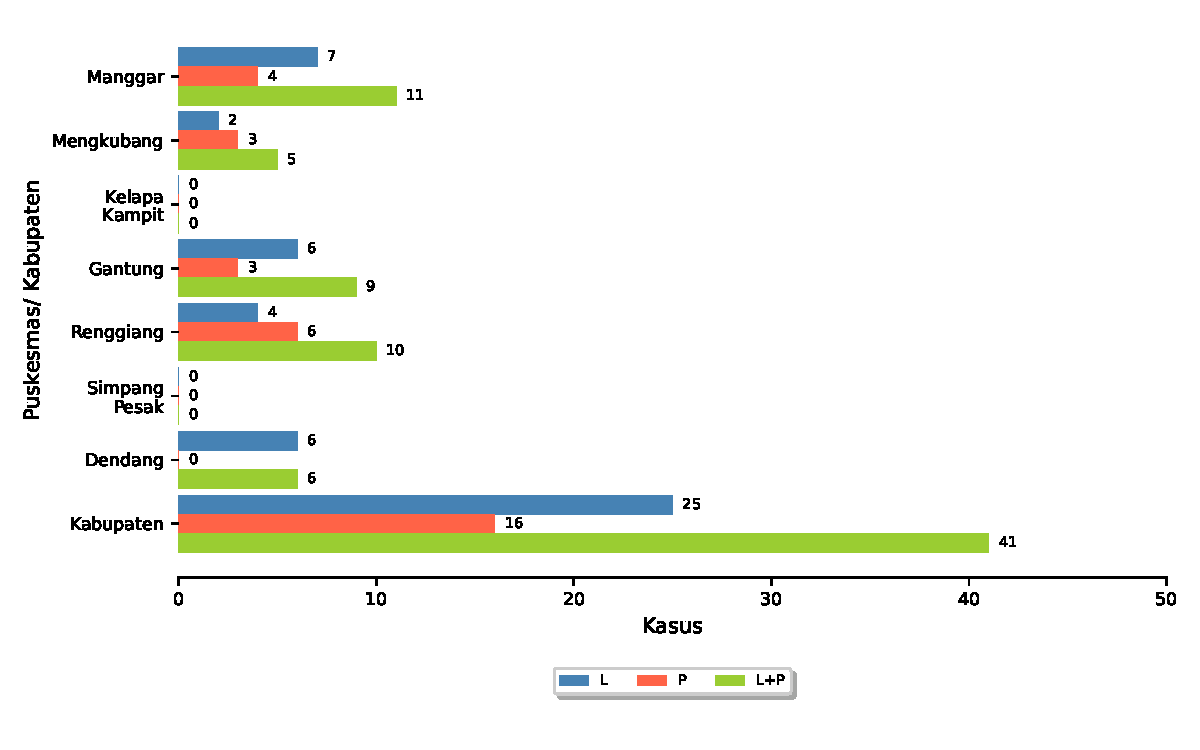
\includegraphics[width=0.9\textwidth]{bab_06/bab_06_10_DBD}
  \caption{Jumlah Kasus DBD di Kab. Belitung Timur Tahun \tP per Puskesmas}
  \label{fig:Jumlah-Kasus-DBD}
\end{figure}

Upaya pemberantasan DBD dititikberatkan pada potensi masyarakat untuk dapat perperan serta dalam pemberantasan sarang nyamuk (gerakan 3M+), juru Pemantau Jentik (Jumantik), serta pengenalan gejala DBD dan penanganannya di rumah tangga.
Dalam rangka penurunan Angka Insiden kasus DBD, pada tahun \tP Dinas Kesehatan Kabupaten Belitung Timur, telah dilaksanakan beberapa program penunjang, antara lain yaitu penyebaran informasi tentang penatalaksanaan kasus DBD, pelacakan kasus DBD, rapat koordinasi, distribusi bahan penunjang, dan lain sebagainya.

\subsection{Penyakit Malaria}
Malaria adalah penyakit infeksi yang disebabkan oleh parasit Plasmodium yang hidup dan berkembang biak dalam sel darah merah manusia, ditularkan oleh nyamuk malaria (\emph{Anopheles sp}) betina.
Malaria dapat menyerang semua orang baik laki-laki ataupun perempuan pada semua golongan umur dari bayi, anak-anak dan orang dewasa.

Angka Kesakitan/ \emph{Annual Parasite Incidence} (API) adalah jumlah penderita positif malaria (dengan pemeriksaan sediaan darah) di suatu wilayah kerja pada kurun waktu
tertentu per 1.000 jumlah penduduk berisiko pada wilayah kurun waktu yang sama.

Pada tahun \tP tidak ditemukan kasus malaria di Kabupaten Belitung Timur sehingga API Kabupaten Belitung Timur pada tahun \tP adalah sebesar 0,00 per 1.000 penduduk.

Penegakan diagnosa penderita secara cepat dan tepat dalam pengobatan merupakan upaya yang sangat penting, dalam rangka pemberantasan penyakit malaria, di samping pengendalian vektor secara potensial.
Kegiatan yang telah dilakukan Dinas Kesehatan Kabupaten Belitung Timur pada tahun \tP adalah antara lain Penemuan Penderita secara aktif (\emph{Active Case Detection}) dan Deteksi Pasif (\emph{Passive Case Detection}), melalui pemeriksaan kesediaan darah, pengobatan penderita, Larvaciding, penyemprotan rumah, pengamatan survei entolomogi, peningkatan kemampuan petugas melalui pelatihan petugas dan magang, rapat koordinasi, pengadaan bahan-bahan penunjang, dan lain sebagainya.

\subsection{Penyakit Filariasis/ Kaki Gajah}
Filariasis (Penyakit Kaki Gajah) adalah penyakit menular yang mengenai saluran dan kelenjar limfe disebabkan oleh cacing filaria (\emph{Wucheria bancrofti}, \emph{Brugia malayi}, \emph{Brugia timori}) dan ditularkan melalui perantaraan nyamuk sebagai vektor.
Penyakit ini bersifat kronis dan bila tidak mendapat pengobatan dapat menimbulkan cacat menetap seumur hidup berupa pembesaran abnormal pada kaki, lengan dan alat kelamin.

Program eliminasi filariasis dilaksanakan atas dasar kesepakatan global WHO tahun 2000 yaitu “\emph{The Global Goal Of Elimination Of Lymphatic Filariasis as a Public Health Problem The Year 2000}”.
Pemberantasan filariasis dilakukan dengan pemutusan mata rantai penularan filariasis, yaitu dengan program Pemberian Obat Pencegahan Massal Filariasis sekali setahun selama 5 tahun berturut-turut.
Program ini juga dikenal dengan Bulan Eliminasi Kaki Gajah (Belkaga), yaitu bulan dimana setiap penduduk kabupaten/ kota endemis Filariasis secara serentak minum obat pencegahan.

Pada tahun \tP ditemukan 1 kasus baru Filariasis di Kabupaten Belitung Timur.
Masih terdapat 11 kasus kronis Filariasis lama pada tahun \tP di Kabupaten Belitung Timur (\autoref{fig:Kasus-Filaria}).

\begin{figure}[H]
  \centering
  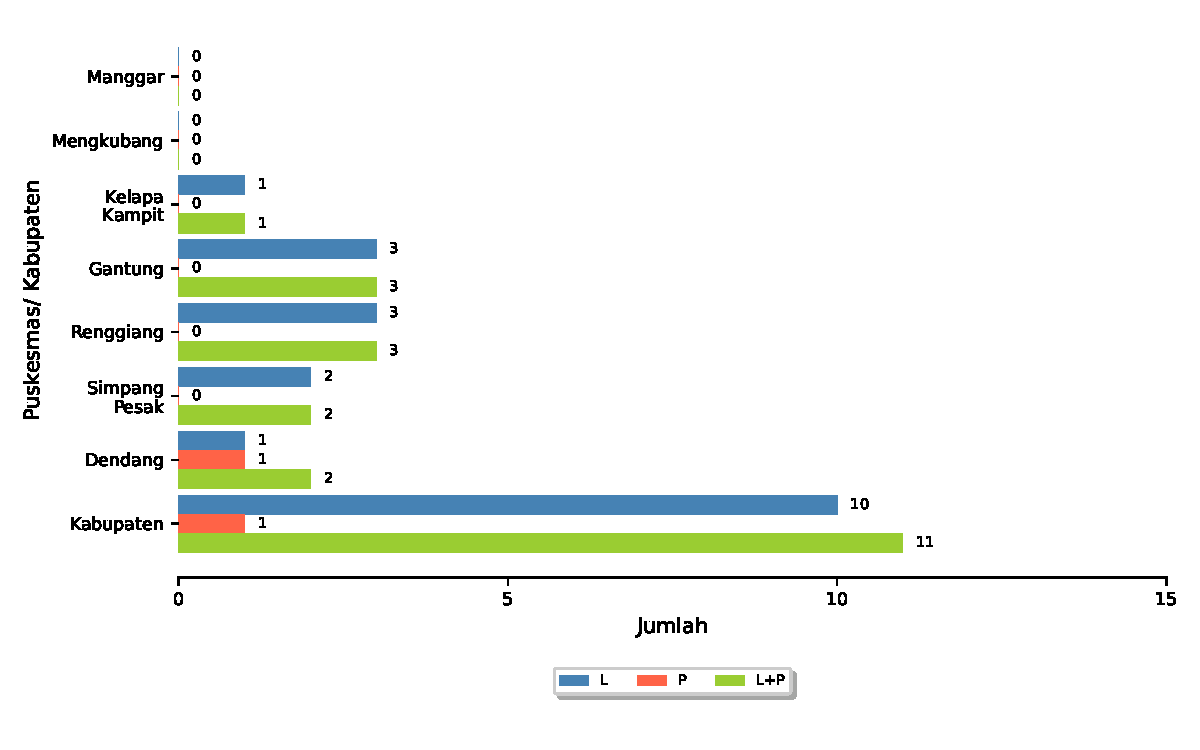
\includegraphics[width=0.85\textwidth]{bab_06/bab_06_12_kasusFilaria}
  \caption{Jumlah Kasus Filaria di Kab. Belitung Timur Tahun \tP per Puskesmas}
  \label{fig:Kasus-Filaria}
\end{figure}

\section[PENGENDALIAN PTM]{PENGENDALIAN PENYAKIT TIDAK MENULAR}
\subsection{Pelayanan Kesehatan Penderita Hipertensi}
Hipertensi adalah keadaan di mana tekanan darah sistolik lebih besar atau sama dengan 140 mmHg dan atau tekanan darah diastolik lebih besar atau sama dengan 90 mmHg.
Setiap penderita hipertensi usia 15 tahun ke atas berhak mendapatkan pelayanan kesehatan sesuai standar sebagai upaya pencegahan sekunder yang meliputi:
\begin{enumerate}
  \item Pengukuran tekanan darah dilakukan minimal satu kali sebulan di fasilitas pelayanan kesehatan; dan
  \item Edukasi perubahan perubahan gaya hidup dan/ atau kepatuhan minum obat.
\end{enumerate}

Dari estimasi penderita hipertensi $\geq$ 15 tahun sebanyak 28.832 orang di Kabupaten Belitung Timur, sebanyak 22.597 orang (78,37\%) mendapatkan pelayanan kesehatan penderita hipertensi (~\autoref{fig:Pelayanan-Hipertensi}).
%Cakupan ini meningkat dari capaian tahun 2021 sebesar 80,19\%.

\begin{figure}[H]
  \centering
  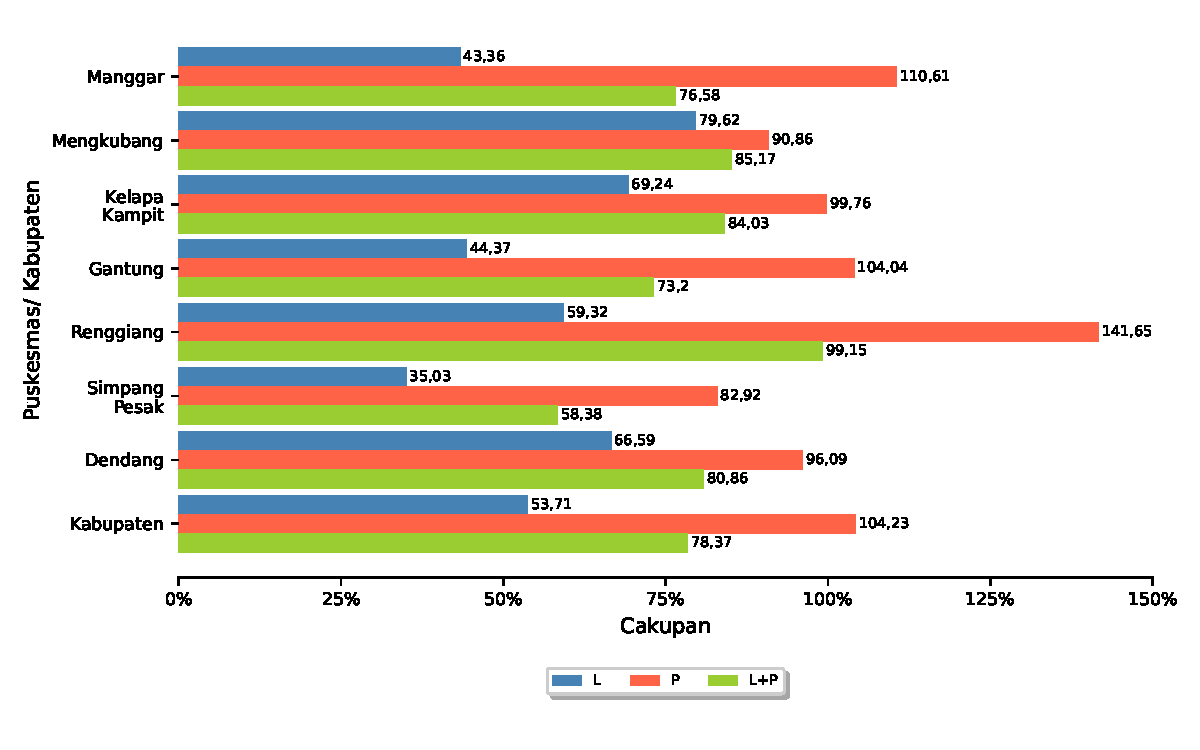
\includegraphics[width=0.85\textwidth]{bab_06/bab_06_13_hipertensi}
  \caption{Pelayanan Kesehatan Penderita Hipertensi di Kab. Belitung Timur Tahun \tP per Puskesmas}
  \label{fig:Pelayanan-Hipertensi}
\end{figure}

\subsection{Pelayanan Kesehatan Penderita Diabetes Melitus (DM)}
Diabetes melitus (DM) adalah penyakit gangguan metabolik menahun akibat pankreas tidak memproduksi cukup insulin (hormon yang mengatur keseimbangan kadar gula darah) atau tubuh tidak dapat menggunakan insulin yang diproduksi secara efektif.
Akibatnya terjadi peningkatan konsentrasi glukosa di dalam darah/ hiperglikemia. 
Hiperglikemia dapat menyebabkan kerusakan berbagai sistem tubuh terutama syaraf dan pembuluh darah. Komplikasi yang umum terjadi akibat diabetes antara lain:
\begin{itemize}
  \item Meningkatkan resiko penyakit jantung dan stroke;
  \item Neuropati (kerusakan syaraf) di kaki yang dapat berujung pada tindakan amputasi;
  \item Retinopati diabetikum, kerusakan pembuluh darah di retina yang mengakibatkan kebutaan;
  \item Meningkatkan resiko penyakit gagal ginjal;
  \item Resiko kematian penderita diabetes secara umum adalah dua kali lipat bukan penderita diabetes;
\end{itemize}
Setiap penderita DM berhak mendapatkan pelayanan kesehatan sesuai standar yang meliputi: edukasi gaya hidup sehat, edukasi aktivitas fisik, edukasi nutrisi medis dan edukasi kepatuhan minum obat.

Dari estimasi penderita DM sebanyak 1.808 orang di Kabupaten Belitung Timur pada tahun \tP, 1.723 orang (95,30\%) mendapatkan pelayanan kesehatan sesuai standar (\autoref{fig:Pelayanan-DM}).
%Cakupan ini meningkat dari capaian tahun 2021 sebesar 89,18\%.

\begin{figure}[H]
  \centering
  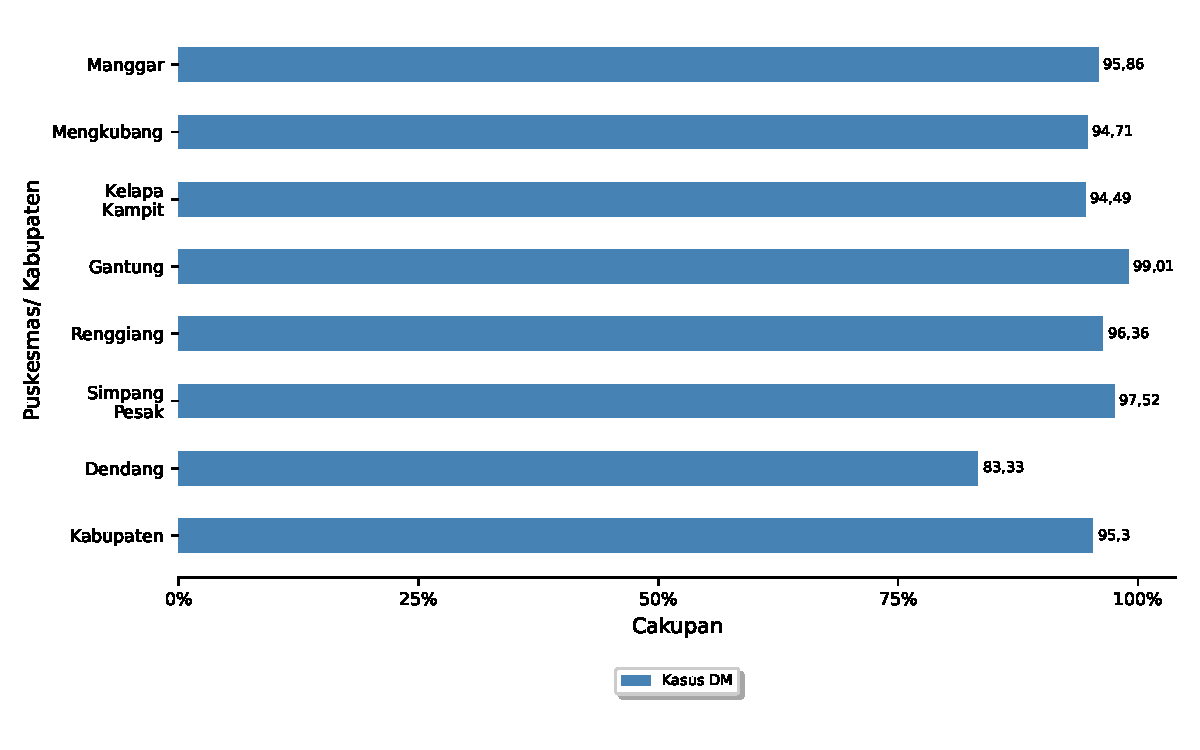
\includegraphics[width=0.85\textwidth]{bab_06/bab_06_14_DM}
  \caption{Cakupan Pelayanan Kesehatan Penderita Diabetes Melitus di Kab. Belitung Timur Tahun \tP per Puskesmas}
  \label{fig:Pelayanan-DM}
\end{figure}

\subsection{Deteksi Dini Kanker Leher Rahim Dengan Metode IVA dan Kanker Payudara Dengan Pemeriksaan Klinis (CBE)}
Kanker adalah pertumbuhan sel yang tidak normal/ terus menerus dan tidak terkendali, dapat merusak jaringan sekitarnya serta dapat menjalar jauh dari tempat asalnya. Sel kanker bersifat ganas dan dapat menyebabkan kematian.
Terdapat berbagai jenis kanker, yang spesifik terjadi pada perempuan adalah kanker leher rahim dan kanker payudara.
Deteksi dini kanker leher rahim dilakukan skrining dengan metode IVA, yaitu inspeksi visual pada seluruh permukaan leher rahim dengan bantuan asam asetat/ cuka yang diencerkan.
Deteksi dini kanker payudara dilakukan skrining dengan metode Pemeriksaan Payudara Klinis (Sadanis)/ \emph{Clinical Breast Examination} (CBE), yaitu pemeriksaan untuk mendeteksi timbulnya kista (massa yang menebal dan berisi cairan) pada payudara.

Cakupan pemeriksaan IVA+ adalah jumlah perempuan usia 30-49 tahun yang dilakukan deteksi dini kanker leher rahim di suatu wilayah pada periode tertentu dibagi jumlah perempuan usia 30-49 tahun pada wilayah dan periode waktu yang sama dikali 100\%.
Dari perkiraan sasaran perempuan usia 30-49 tahun sebanyak 19.653 orang, yang dilakukan pemeriksaan IVA adalah sebanyak 3.311 orang atau sebesar 16,85\% (\autoref{fig:Pemeriksaan-IVA}).
Sebanyak 5 orang atau 0,15\% ditemukan IVA positif.

\begin{figure}[H]
  \centering
  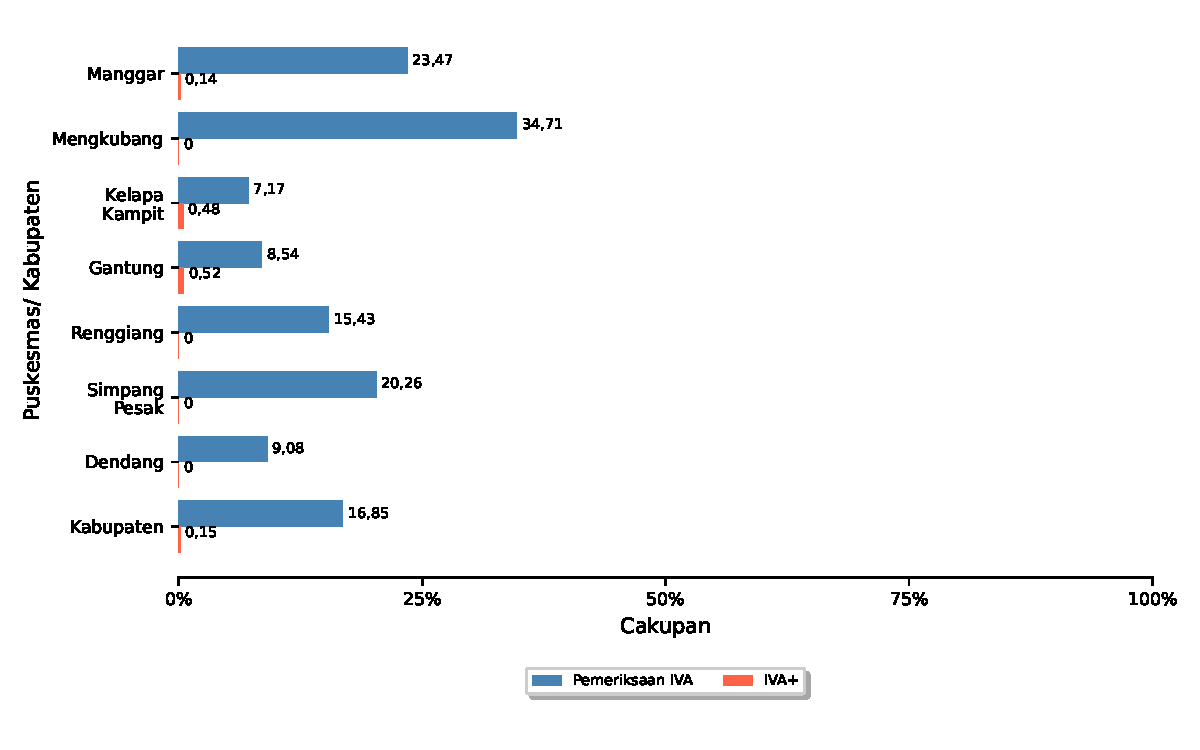
\includegraphics[width=0.9\textwidth]{bab_06/bab_06_15a_IVA}
  \caption{Cakupan Pemeriksaan IVA+ di Kab. Belitung Timur Tahun \tP per Puskesmas}
  \label{fig:Pemeriksaan-IVA}
\end{figure}

Cakupan pemeriksaan sadanis adalah jumlah perempuan usia 30-49 tahun yang dilakukan deteksi dini kanker payudara di suatu wilayah pada periode tertentu dibagi jumlah perempuan usia 30-49 tahun pada wilayah dan periode waktu yang sama dikali 100\%.
Dari perkiraan sasaran perempuan usia 30-49 tahun sebanyak 19.653 orang, yang dilakukan pemeriksaan sadanis adalah sebanyak 2.927 orang atau sebesar 14,89\% (\autoref{fig:Pemeriksaan-IVA}).

\begin{figure}[H]
	\centering
	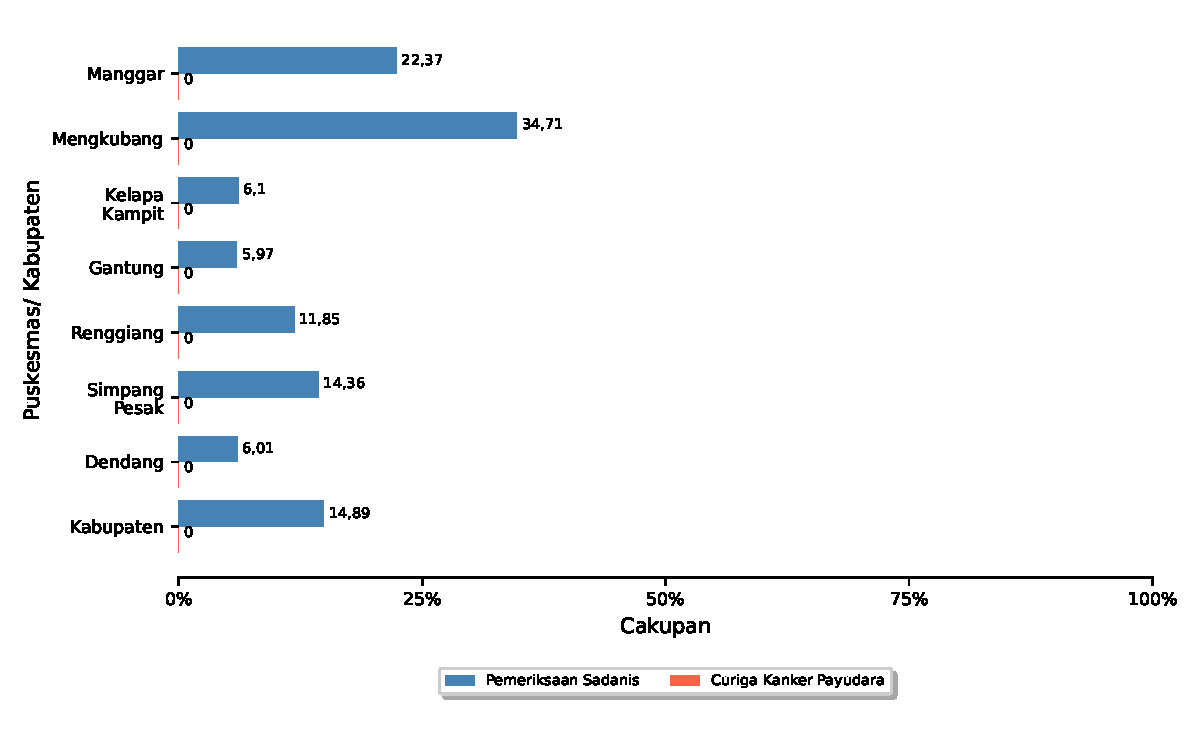
\includegraphics[width=0.9\textwidth]{bab_06/bab_06_15b_sadanis}
	\caption{Cakupan Pemeriksaan Sadanis di Kab. Belitung Timur Tahun \tP per Puskesmas}
	\label{fig:Pemeriksaan-Sadanis}
\end{figure}

\subsection{Pelayanan Kesehatan Orang dengan Gangguan Jiwa Berat (ODGJB)}
Orang dengan Gangguan Jiwa Berat (ODGJB) adalah orang dengan gangguan Psikotik akut dan Skizofrenia.
Psikotik akut adalah gangguan jiwa dengan tanda tidak mampu menilai kenyataan yang terjadi, misalnya terdapat halusinasi, waham atau perilaku kacau/ aneh.
Skizofrenia adalah gangguan jiwa berat yang ditandai dengan gangguan penilaian realita (waham dan halusinasi).
Waham adalah suatu keadaan dimana suatu kepercayaan yang salah, menetap dalam pikiran yang tidak sesuai dengan fakta dan tidak bisa dikoreksi.

Pelayanan kesehatan Orang Dengan Gangguan Jiwa Berat (ODGJB) adalah pelayanan promotif dan preventif yang diberikan oleh pemerintah daerah kabupaten/kota pada orang dengan gangguan Psikotik akut dan Skizofrenia untuk mengoptimalkan derajat kesehatan jiwanya agar dapat berfungsi dalam kehidupan sehari-hari, mencegah terjadinya kekambuhan dan pemasungan.
Setiap ODGJB berhak mendapatkan pelayanan kesehatan sesuai standar, yaitu sesuai Pedoman Penggolongan Diagnosis Gangguan Jiwa-III (PPDGJ-III/ICD-X), mendapat kunjungan rumah dari petugas dan edukasi kepatuhan minum obat sesuai anjuran dokter.

Sebanyak 300 penderita ODGJB ditemukan di Kabupaten Belitung Timur pada tahun \tP (\autoref{fig:Pelayanan-ODGJB}).
Dari jumlah tersebut, sebanyak 300 orang (100\%) telah mendapatkan perawatan sesuai standar.

\begin{figure}[H]
	\centering
	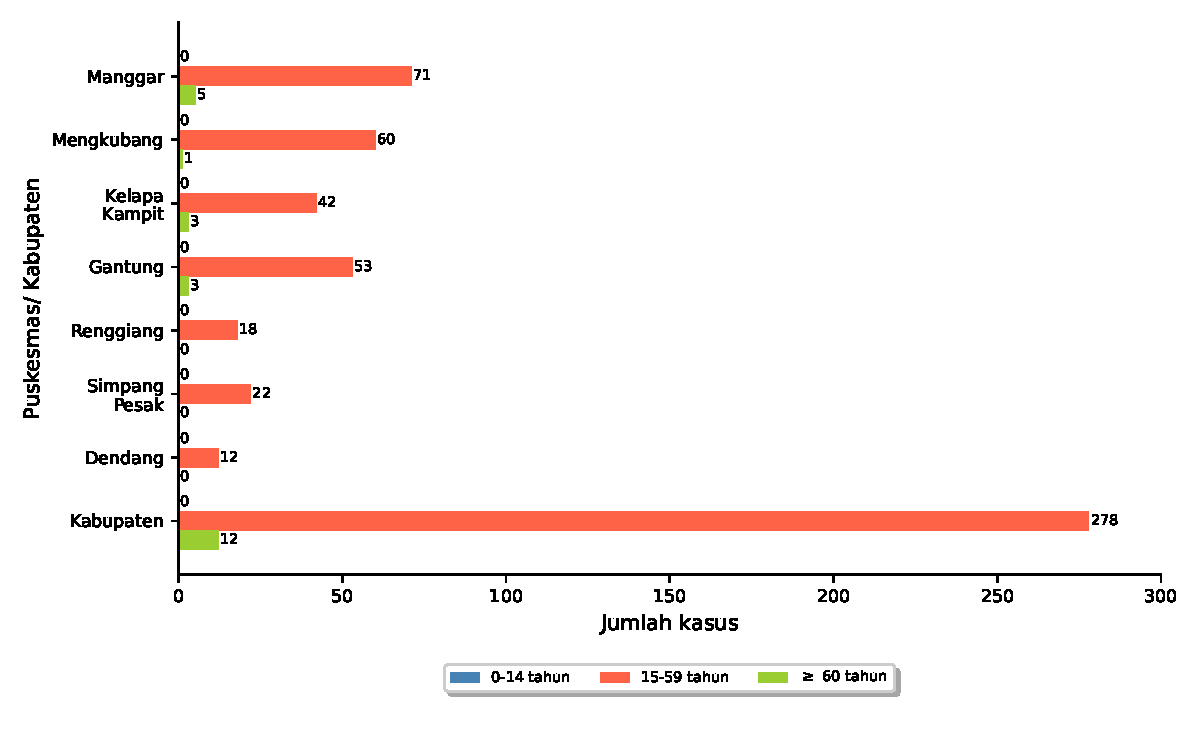
\includegraphics[width=0.85\textwidth]{bab_06/bab_06_16a_skizofrenia}
	\caption{Jumlah Kasus Skizofrenia di Kab. Belitung Timur Tahun \tP per Puskesmas}
	\label{fig:Kasus-Skizofrenia}
\end{figure}

\begin{figure}[H]
	\centering
	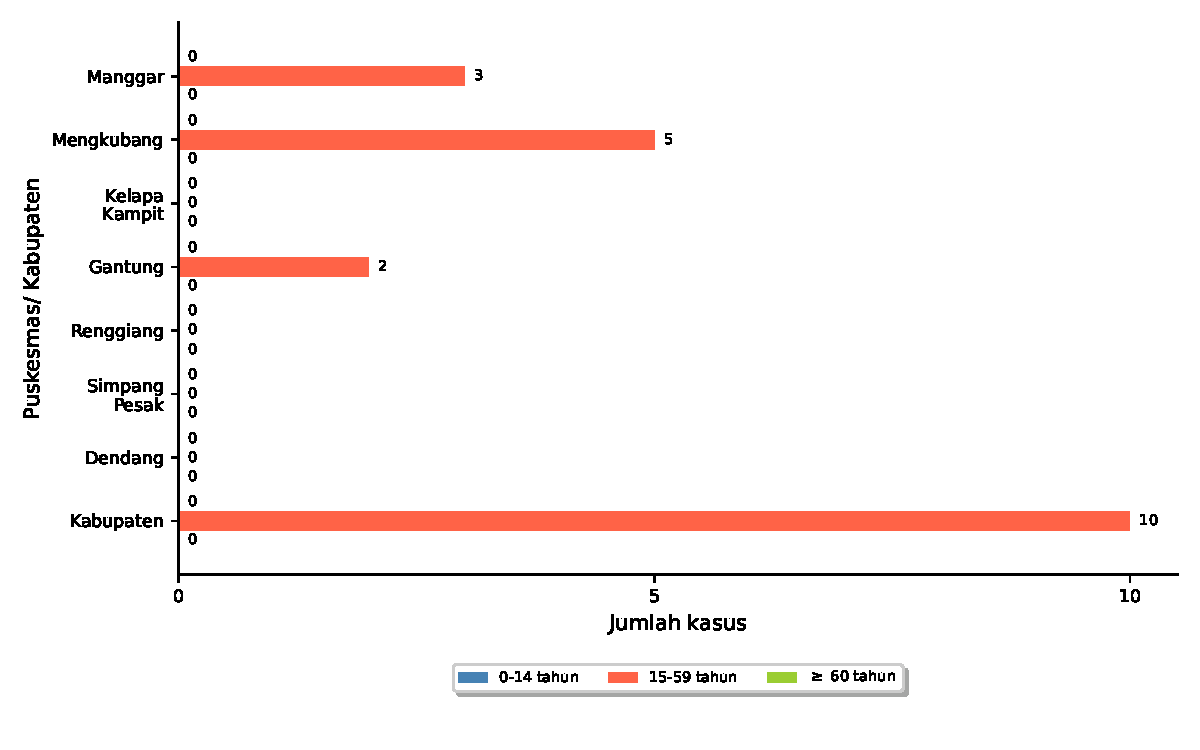
\includegraphics[width=0.85\textwidth]{bab_06/bab_06_16b_psikotik}
	\caption{Jumlah Kasus Psikotik di Kab. Belitung Timur Tahun \tP per Puskesmas}
	\label{fig:Kasus-Psikotik}
\end{figure}

\begin{figure}[H]
  \centering
  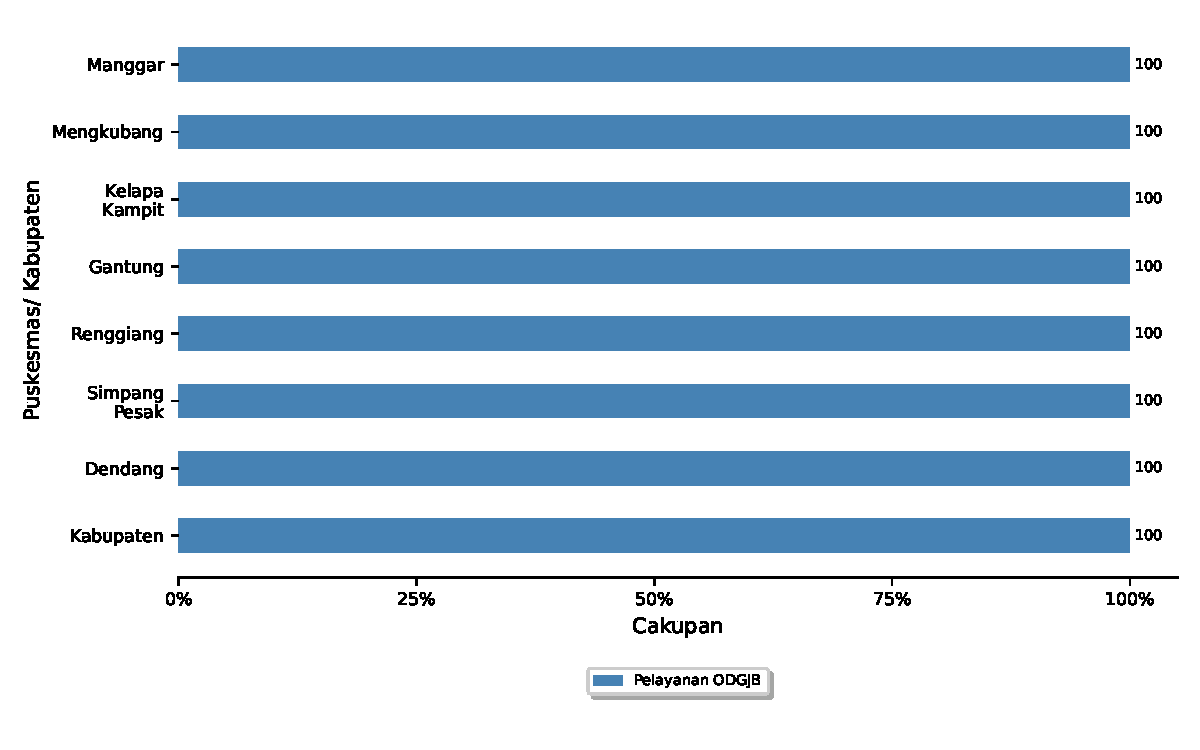
\includegraphics[width=0.85\textwidth]{bab_06/bab_06_16c_pelayananODGJB}
  \caption{Cakupan Pelayanan Kesehatan Orang Dengan Gangguan Jiwa Berat (ODGJB) di Kab. Belitung Timur Tahun \tP per Puskesmas}
  \label{fig:Pelayanan-ODGJB}
\end{figure}

\section[INFEKSI EMERGING]{INFEKSI EMERGING}
Infeksi \textit{emerging} atau \textit{Emerging Infectious Diseases} (EIDs) adalah penyakit yang muncul dan menyerang suatu populasi untuk pertama kalinya, atau telah ada sebelumnya namun meningkat dengan sangat cepat, baik dalam hal jumlah kasus baru didalam suatu populasi, atau penyebarannya ke daerah geografis yang baru.
Yang juga dikelompokkan dalam EIDs adalah penyakit yang pernah terjadi di suatu daerah di masa lalu, kemudian menurun atau telah dikendalikan, namun kemudian dilaporkan lagi dalam jumlah yang meningkat.

Kadang-kadang sebuah penyakit lama muncul dalam bentuk klinis baru, yang bisa jadi lebih parah atau fatal.
Penyakit ini disebut dengan penyakit lama (\textit{re-emerging}).

\subsection{Coronavirus Disease-2019 (COVID-19)}
Coronavirus merupakan keluarga besar virus yang menyebabkan penyakit pada manusia dan hewan.
Pada manusia biasanya menyebabkan penyakit infeksi saluran pernapasan, mulai flu biasa hingga penyakit yang serius seperti \textit{Middle East Respiratory Syndrome} (MERS) dan Sindrom Pernafasan Akut Berat/ \textit{Severe Acute Respiratory Syndrome} (SARS).
\textit{Severe Acute Respiratory Syndrome Coronavirus} 2 (SARS-COV2) adalah Coronavirus jenis baru yang ditemukan pada manusia sejak kejadian luar biasa muncul di Wuhan, Cina, pada Desember 2019, dan menyebabkan penyakit \textit{Coronavirus Disease}-2019 (COVID-19).

Gejala umum COVID-19 berupa demam $\geq$ 38\textdegree C, batuk kering, dan sesak napas.
COVID-19 dapat menyebabkan gejala ringan hingga berat.
Sekitar 80\% kasus dengan gejala ringan (pilek, sakit tenggorokan, batuk, dan demam) dapat pulih tanpa perlu perawatan khusus.
Namun, sekitar 1 dari setiap 5 orang mungkin akan menderita sakit yang parah, seperti disertai pneumonia atau kesulitan bernafas, yang biasanya muncul secara bertahap.
Orang yang berusia lanjut, dan orang-orang dengan kondisi medis yang sudah ada sebelumnya/ \emph{pre-existing condition} (seperti diabetes, tekanan darah tinggi dan penyakit jantung, paru-paru, atau kanker) biasanya lebih rentan untuk menjadi sakit parah.
COVID-19 dapat menyebabkan kematian.

\subsubsection{Morbiditas dan mortalitas}
Jumlah kasus COVID-19 di Kabupaten Belitung Timur pada tahun \tP adalah sebanyak 3 kasus, turun drastis dari periode 2022 (614 kasus). 
Dari jumlah tersebut tidak ada penderita COVID-19 meninggal di Kabupaten Belitung Timur pada tahun \tP.

\begin{figure}[H]
	\centering
	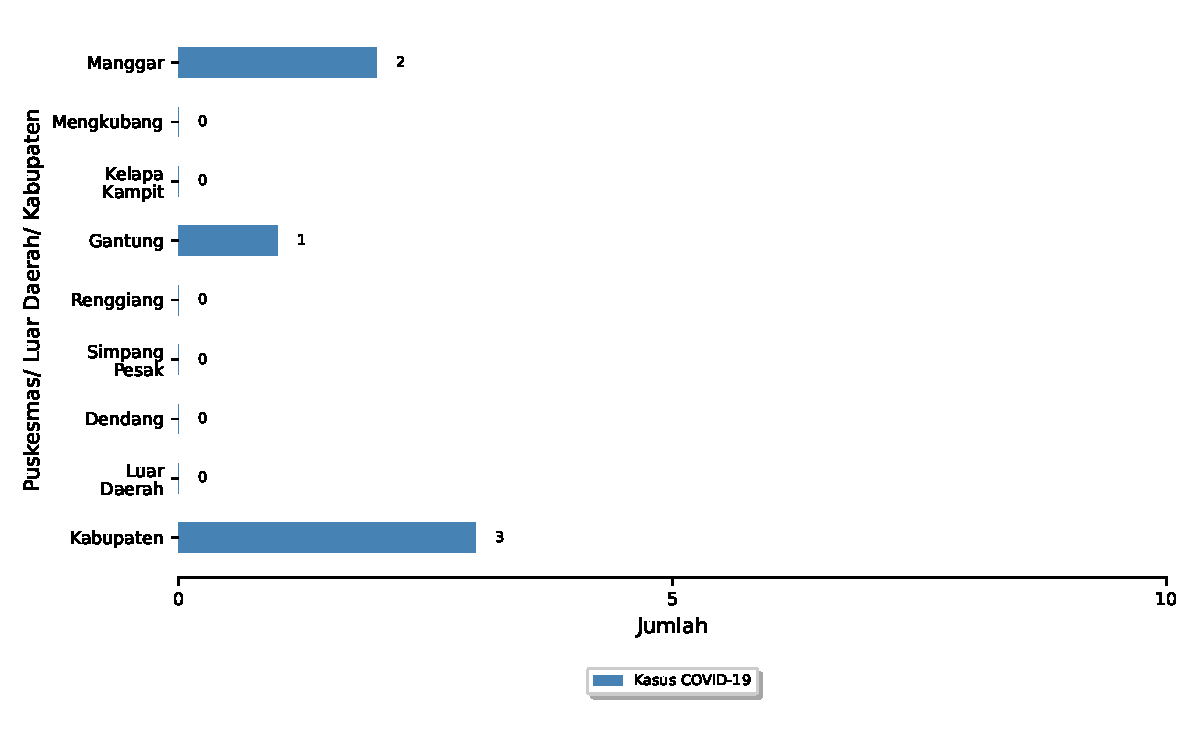
\includegraphics[width=0.85\textwidth]{bab_06/bab_06_17a_kasusCovid}
	\caption{Jumlah Kasus COVID-19 di Kab. Belitung Timur Tahun \tP per Puskesmas}
	\label{fig:Kasus-COVID}
\end{figure}

\begin{figure}[H]
	\centering
	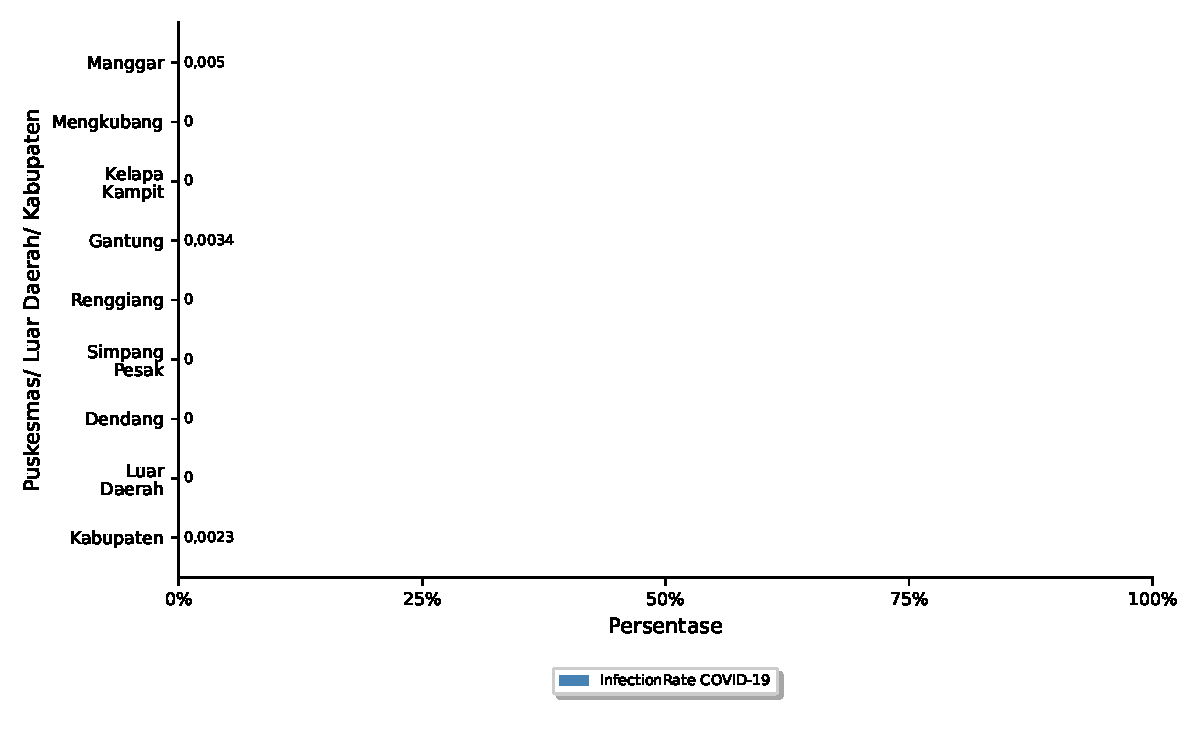
\includegraphics[width=0.85\textwidth]{bab_06/bab_06_17b_infectionRateCovid}
	\caption{\emph{Infection Rate} COVID-19 di Kab. Belitung Timur Tahun \tP per Puskesmas}
	\label{fig:IR-COVID}
\end{figure}

\begin{figure}[H]
	\centering
	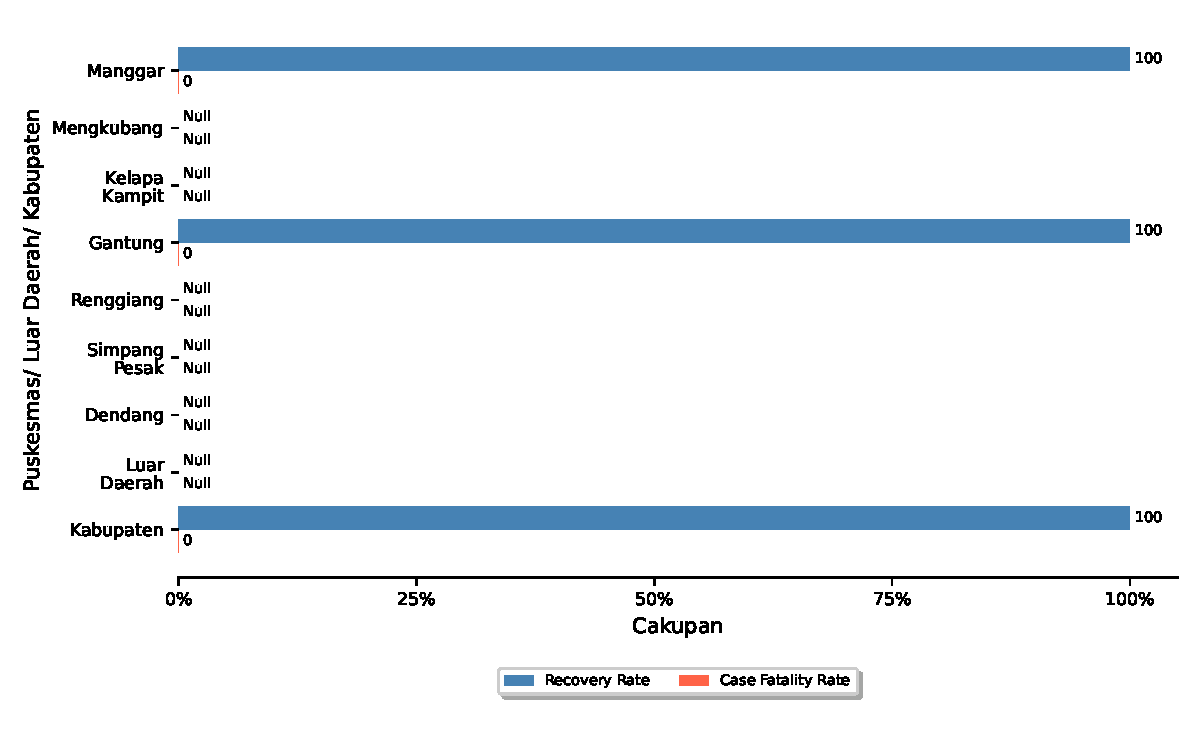
\includegraphics[width=0.85\textwidth]{bab_06/bab_06_17c_kasusCovidKesembuhan}
	\caption{\emph{Recovery Rate} dan \emph{Case Fatality Rate} di Kab. Belitung Timur Tahun \tP per Puskesmas}
	\label{fig:RR-COVID}
\end{figure}

\begin{figure}[H]
	\centering
	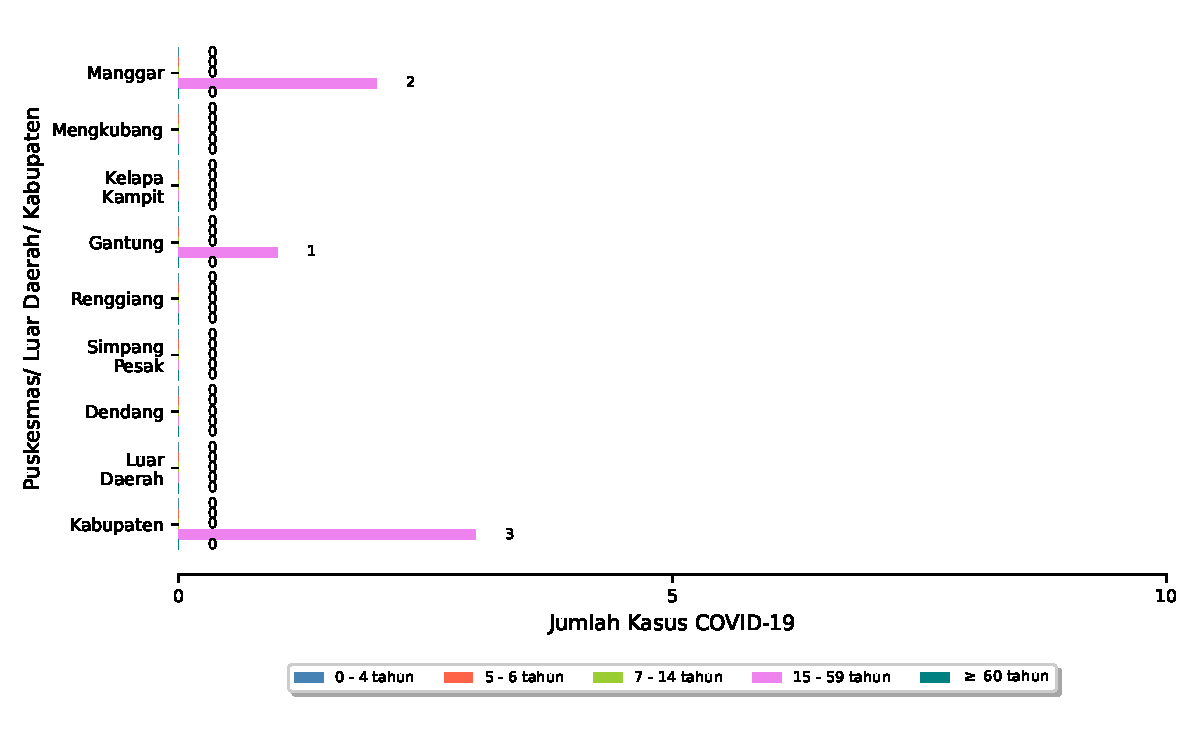
\includegraphics[width=0.85\textwidth]{bab_06/bab_06_17d_kasusCovidPerUmur}
	\caption{Jumlah Kasus COVID-19 Menurut Kelompok Umur di Kab. Belitung Timur Tahun \tP per Puskesmas}
	\label{fig:COVID-per-umur}
\end{figure}

\begin{figure}[H]
	\centering
	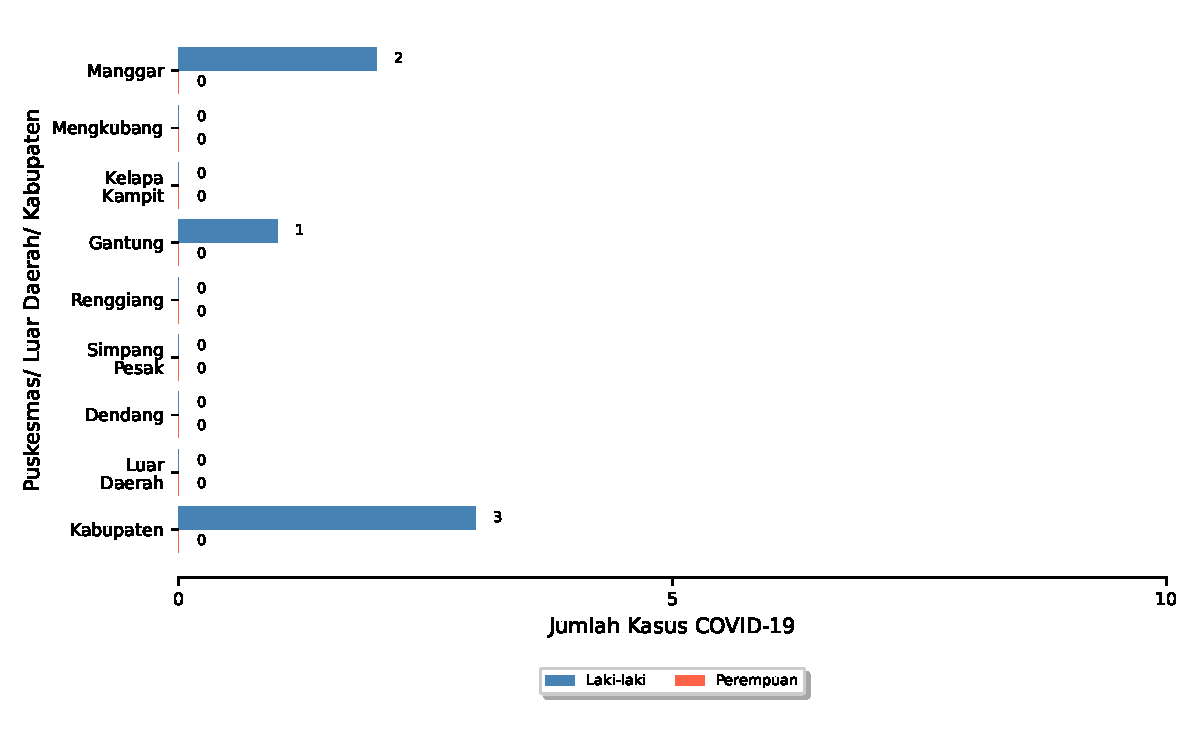
\includegraphics[width=0.85\textwidth]{bab_06/bab_06_17e_kasusCovidPerJK}
	\caption{Jumlah Kasus COVID-19 Menurut Jenis Kelamin di Kab. Belitung Timur Tahun \tP per Puskesmas}
	\label{fig:COVID-per-JK}
\end{figure}

\subsubsection{Upaya pengendalian}
Pengendalian penyebaran COVID-19 dilakukan dengan sosialisasi 5M (Mencuci tangan, Memakai masker, Menjaga jarak, Menjauhi kerumunan, Mengurangi mobilitas), protokol isolasi mandiri dan isolasi terpadu suspek dan positif COVID-19, serta vaksinasi massal. Vaksinasi massal dilakukan sejak bulan Januari 2021 secara bertahap sesuai dengan ketersediaan vaksin yang didistribusikan oleh Kementerian Kesehatan Republik Indonesia. Tahapan vaksinasi dimulai dengan sasaran SDM Kesehatan pada bulan Januari 2021, sasaran pelayan publik pada bulan Maret 2021, sasaran penduduk lanjut usia pada bulan Maret 2021, sasaran masyarakat umum pada bulan Juni 2021, sasaran remaja pada bulan Juli 2021, dan sasaran anak-anak pada bulan Desember 2021.

Vaksinasi COVID-19 dosis 1 dan 2 di Kabupaten Belitung Timur pada tahun \tP tidak lagi dilakukan dikarenakan penurunan status Pandemi COVID-19 menjadi Endemik.

%\begin{figure}[H]
%	\centering
%	\includegraphics[width=0.85\textwidth]{bab_06/bab_06_17f_vaksinCovidDos1}
%	\caption{Cakupan Vaksin COVID-19 Dosis 1 di Kab. Belitung Timur Tahun \tP per Puskesmas}
%	\label{fig:vaksin-COVID-dosis-1}
%\end{figure}
%
%\begin{figure}[H]
%	\centering
%	\includegraphics[width=0.85\textwidth]{bab_06/bab_06_17g_vaksinCovidDos2}
%	\caption{Cakupan Vaksin COVID-19 Dosis 2 di Kab. Belitung Timur Tahun \tP per Puskesmas}
%	\label{fig:vaksin-COVID-dosis-2}
%\end{figure}